\documentclass{beamer}
\usepackage[utf8]{inputenc}
\usepackage{mystyle} % See mystyle.sty for packages and own commands
%------------------------------------------------------------
%Title page
\title[Post-processing of an 8-node Brick Element]{Post-processing of an 8-node Brick Element \small{(using python)}}
\subtitle{Assignment 4}
\titlegraphic{
\includegraphics[height=0.85cm]{Logos/iitmlogo.png}}
\author[Gaddam Shiva Kumar]{Gaddam Shiva Kumar (MM22D014)}
\institute[]{ME7227 : Nonlinear Finite Element Analysis of Solid Continua}
\date{\today}

%---------------------TITLE PAGE---------------------------------------
\begin{document}
\begin{frame}
\maketitle
\end{frame}
%------------------------------------------------------------

% \logo{
\includegraphics[height=1cm]{Logos/circlelogo.png}~%
% }


%===================================================================
\section{Introduction}

% \begin{frame}
% \frametitle{Table of Contents}
% \tableofcontents
% \end{frame}

\begin{frame}{Introduction}{The Problem Definition}
    
\end{frame}

\begin{frame}{Introduction}{Steps involved - Method-I}
    
\end{frame}

\begin{frame}{Introduction}{Steps involved - Method-II(time integration)}
    
\end{frame}

\begin{frame}{Introduction}{Steps involved - Method-II(time integration)}
    
\end{frame}

%===================================================================
\section{Problem 1}

\begin{frame}{Problem 1 - Translation}{Deformation and Stress vs Strain at t = 0 sec}
    \vspace{-1em}
    \scriptsize $$x_1 = X_1+t,\ x_2 = X_2+t,\ x_3 = X_3$$
    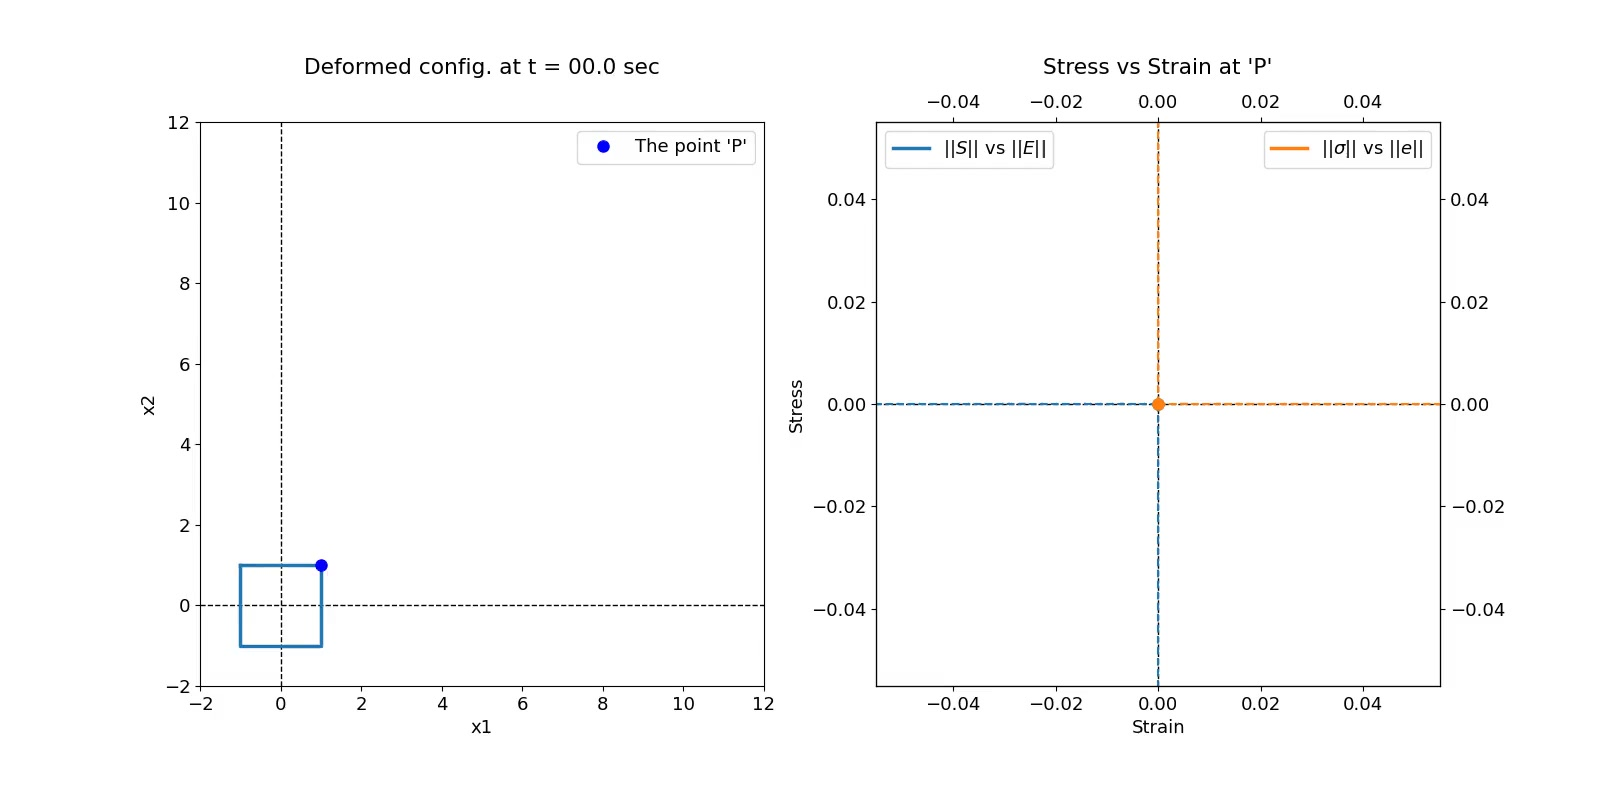
\includegraphics[width=\textwidth, trim={4.5cm 2cm 3cm 1cm}, clip]{Plots/itranslation.jpg}
\end{frame}

\begin{frame}{Problem 1 - Translation}{Deformation and Stress vs Strain at t = 10 sec}
    \vspace{-1em}
    \scriptsize $$x_1 = X_1+t,\ x_2 = X_2+t,\ x_3 = X_3$$
    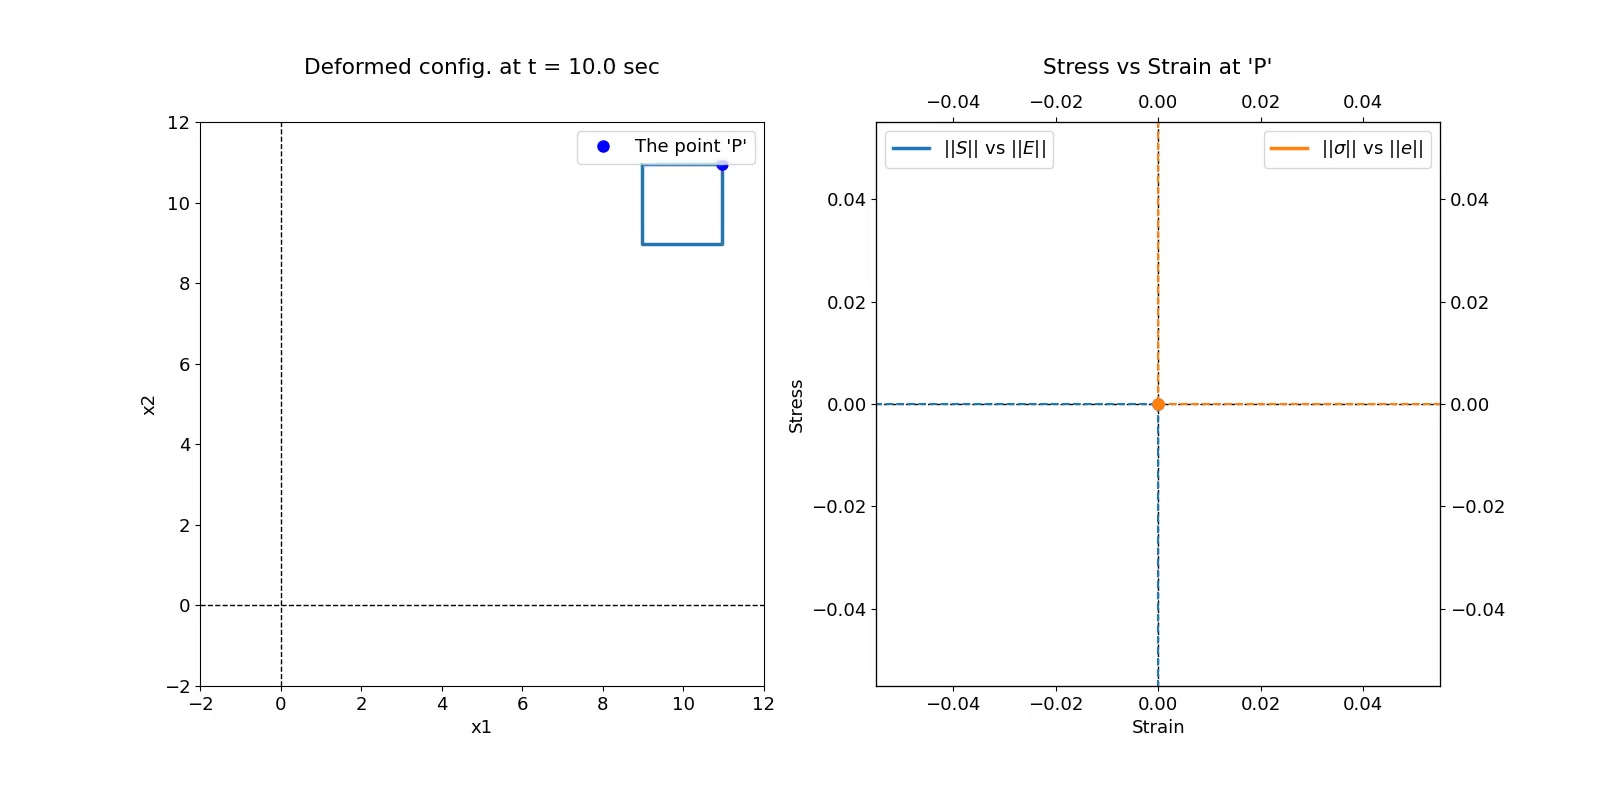
\includegraphics[width=\textwidth, trim={4.5cm 2cm 3cm 1cm}, clip]{Plots/translation.jpg}
\end{frame}

\begin{frame}{Problem 1 - Translation}{Method-I vs Method-II(time integration)}
    \vspace{-2em}
    \begin{columns}
        \column[t]{0.48\textwidth}
        \begin{block}{\footnotesize Method-I}
            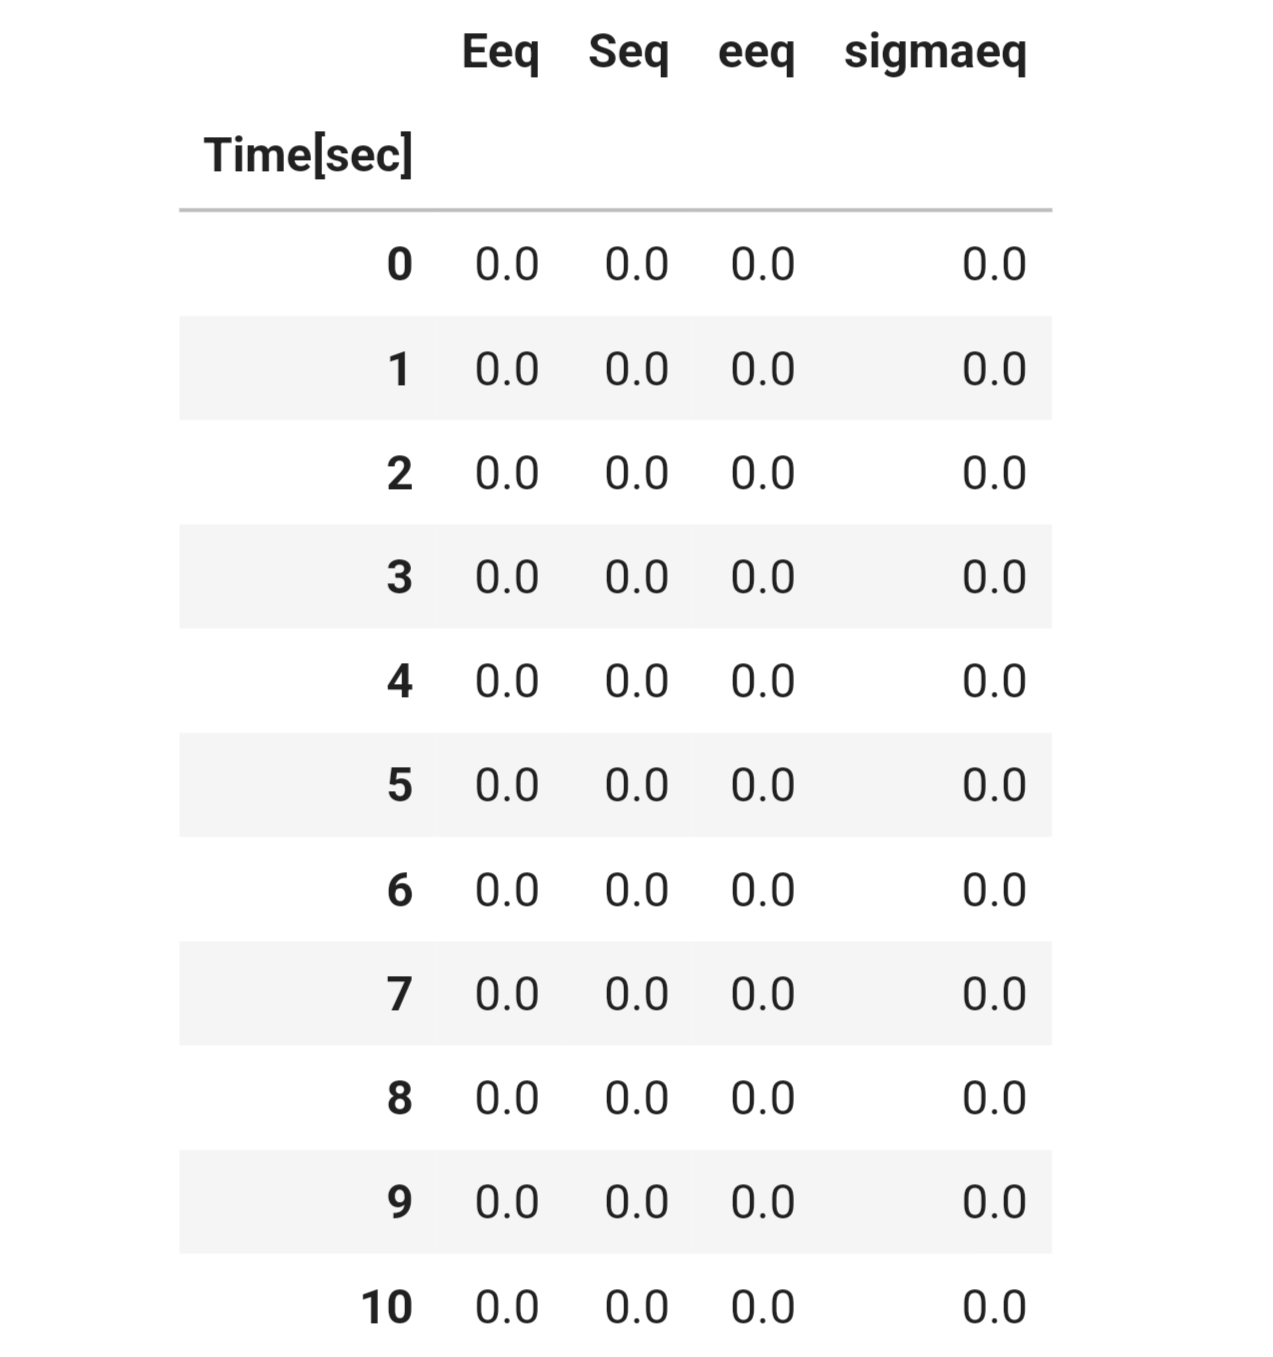
\includegraphics[width=\textwidth]{Values/m2t1.png}
        \end{block}
        \column[t]{0.48\textwidth}
        \begin{block}{\footnotesize Method-II(time integration)}
            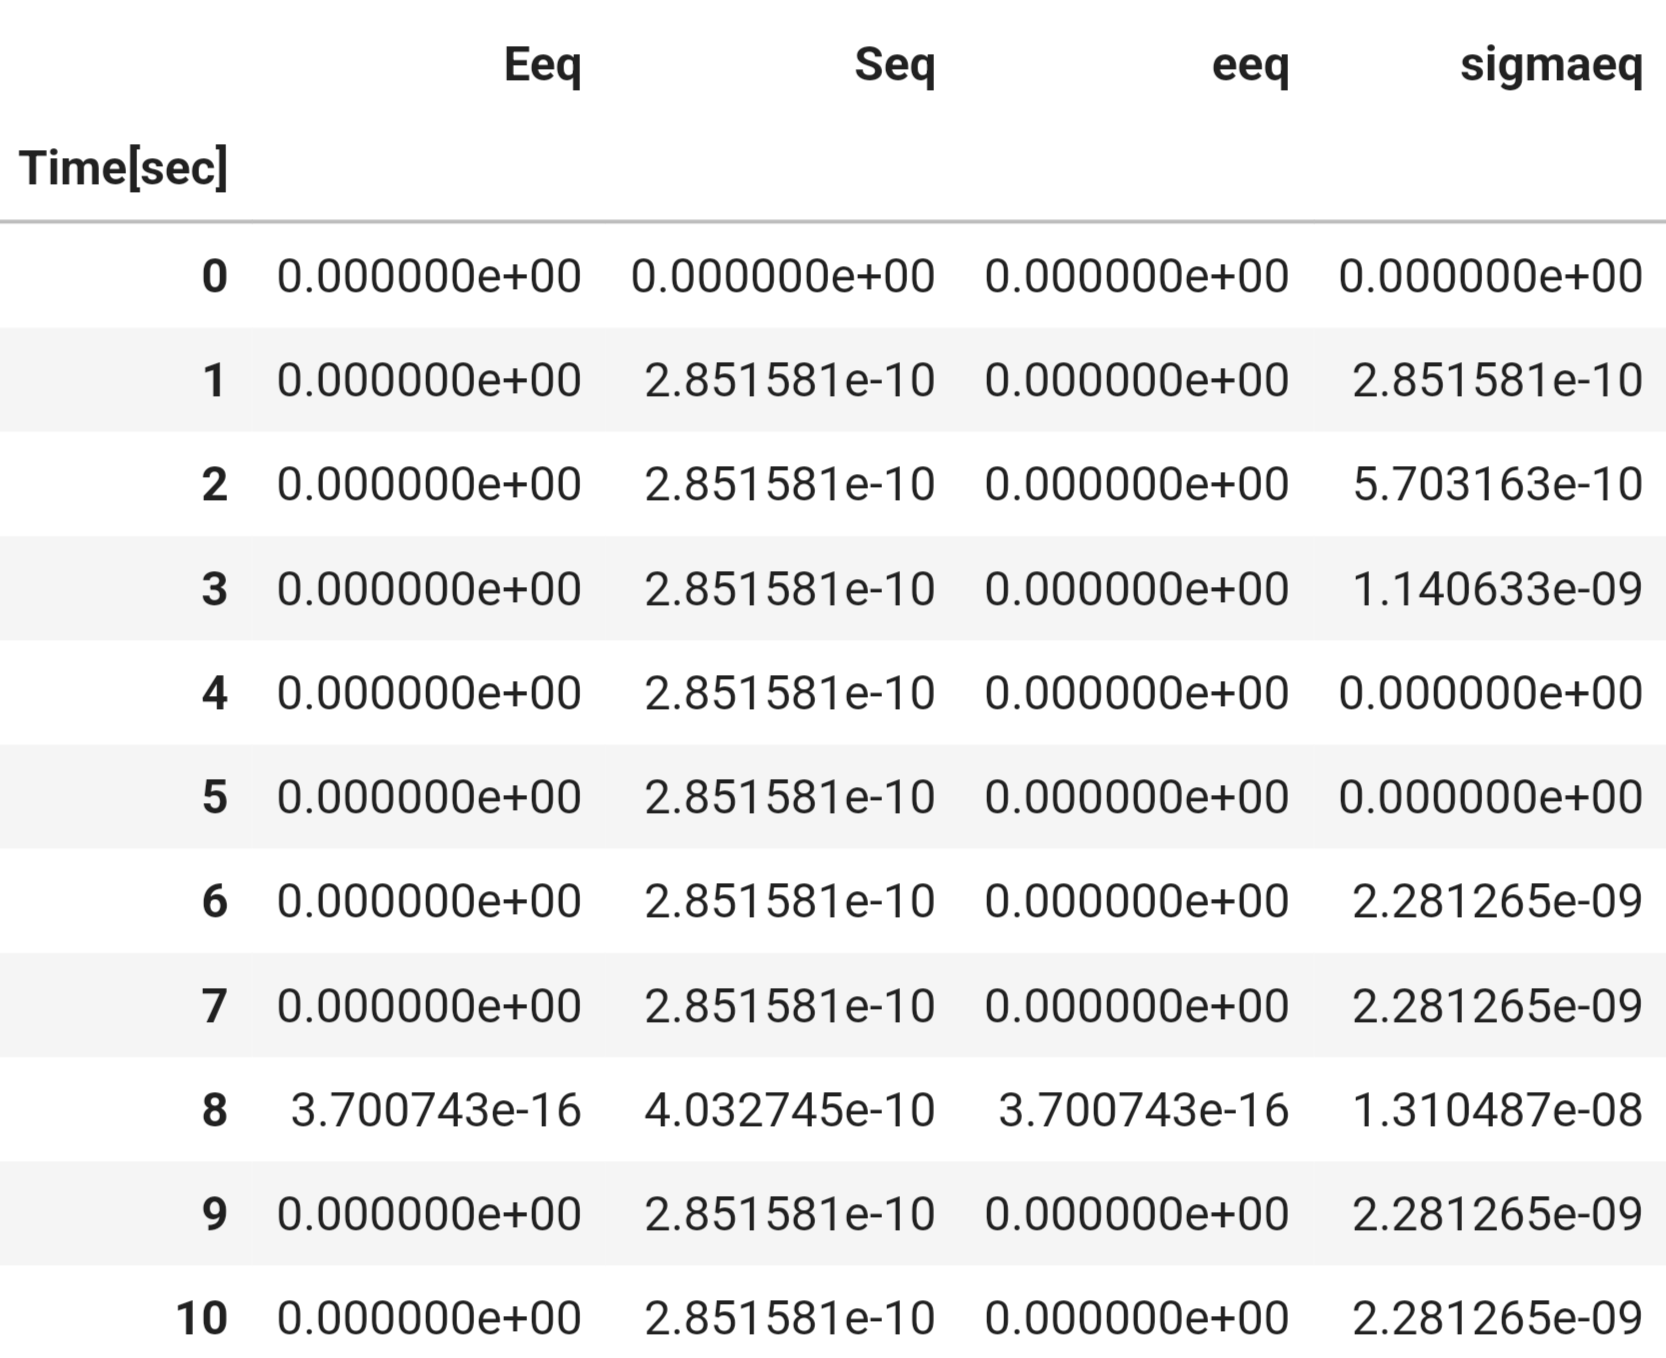
\includegraphics[width=\textwidth]{Values/m1t1.png}
        \end{block}
    \end{columns}
\end{frame}

%===================================================================
\section{Problem 2}

\begin{frame}{Problem 2 - Rotation}{Deformation and Stress vs Strain at t = 0 sec}
    \vspace{-2em}
    \scriptsize $$x_1 = X_1\cos\omega t - X_2\sin\omega t,\ x_2 = X_1\sin\omega t + X_2\cos\omega t,\ x_3 = X_3;\ \ \omega t = 90^o \implies \omega = 9^o$$
    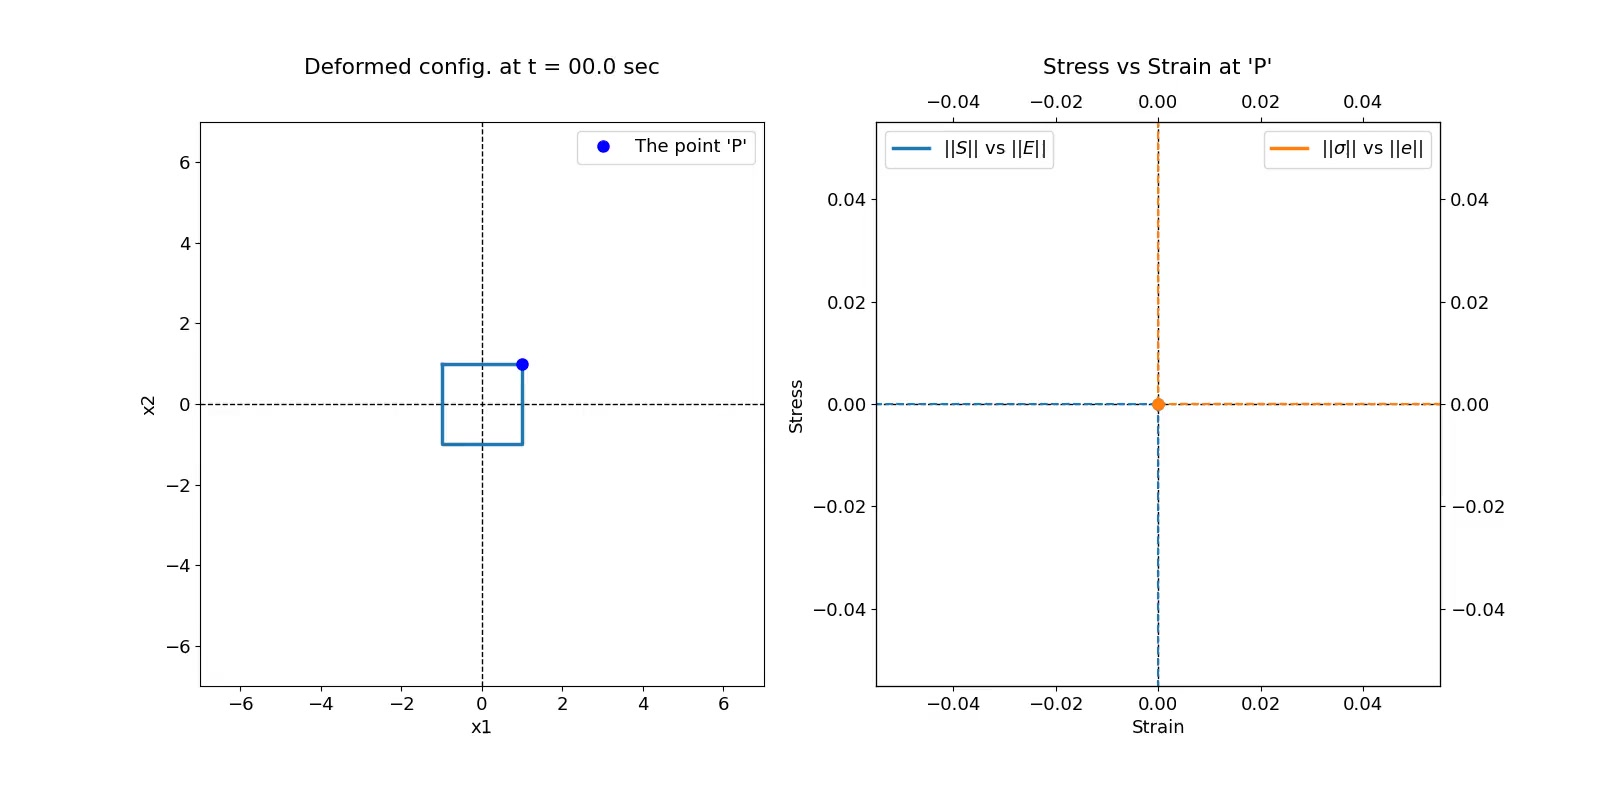
\includegraphics[width=\textwidth, trim={4.5cm 2cm 3cm 1cm}, clip]{Plots/irotation.jpg}
\end{frame}

\begin{frame}{Problem 2 - Rotation}{Deformation and Stress vs Strain at t = 10 sec}
    \vspace{-2em}
    \scriptsize $$x_1 = X_1\cos\omega t - X_2\sin\omega t,\ x_2 = X_1\sin\omega t + X_2\cos\omega t,\ x_3 = X_3;\ \ \omega t = 90^o \implies \omega = 9^o$$
    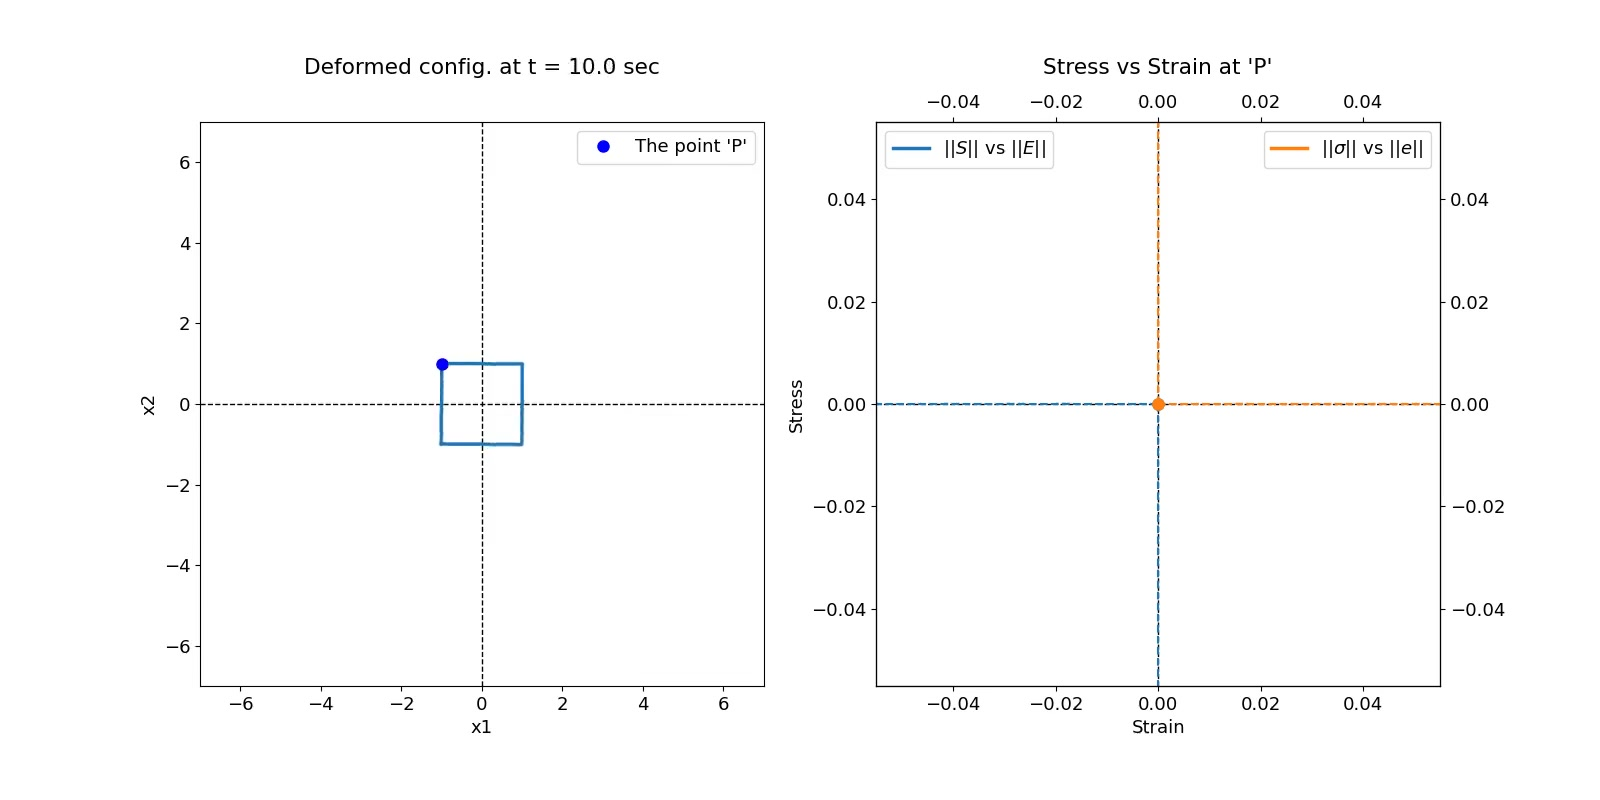
\includegraphics[width=\textwidth, trim={4.5cm 2cm 3cm 1cm}, clip]{Plots/rotation.jpg}
\end{frame}

\begin{frame}{Problem 2 - Rotation}{Method-I vs Method-II(time integration)}
    \vspace{-2em}
    \begin{columns}
        \column[t]{0.48\textwidth}
        \begin{block}{\footnotesize Method-I}
            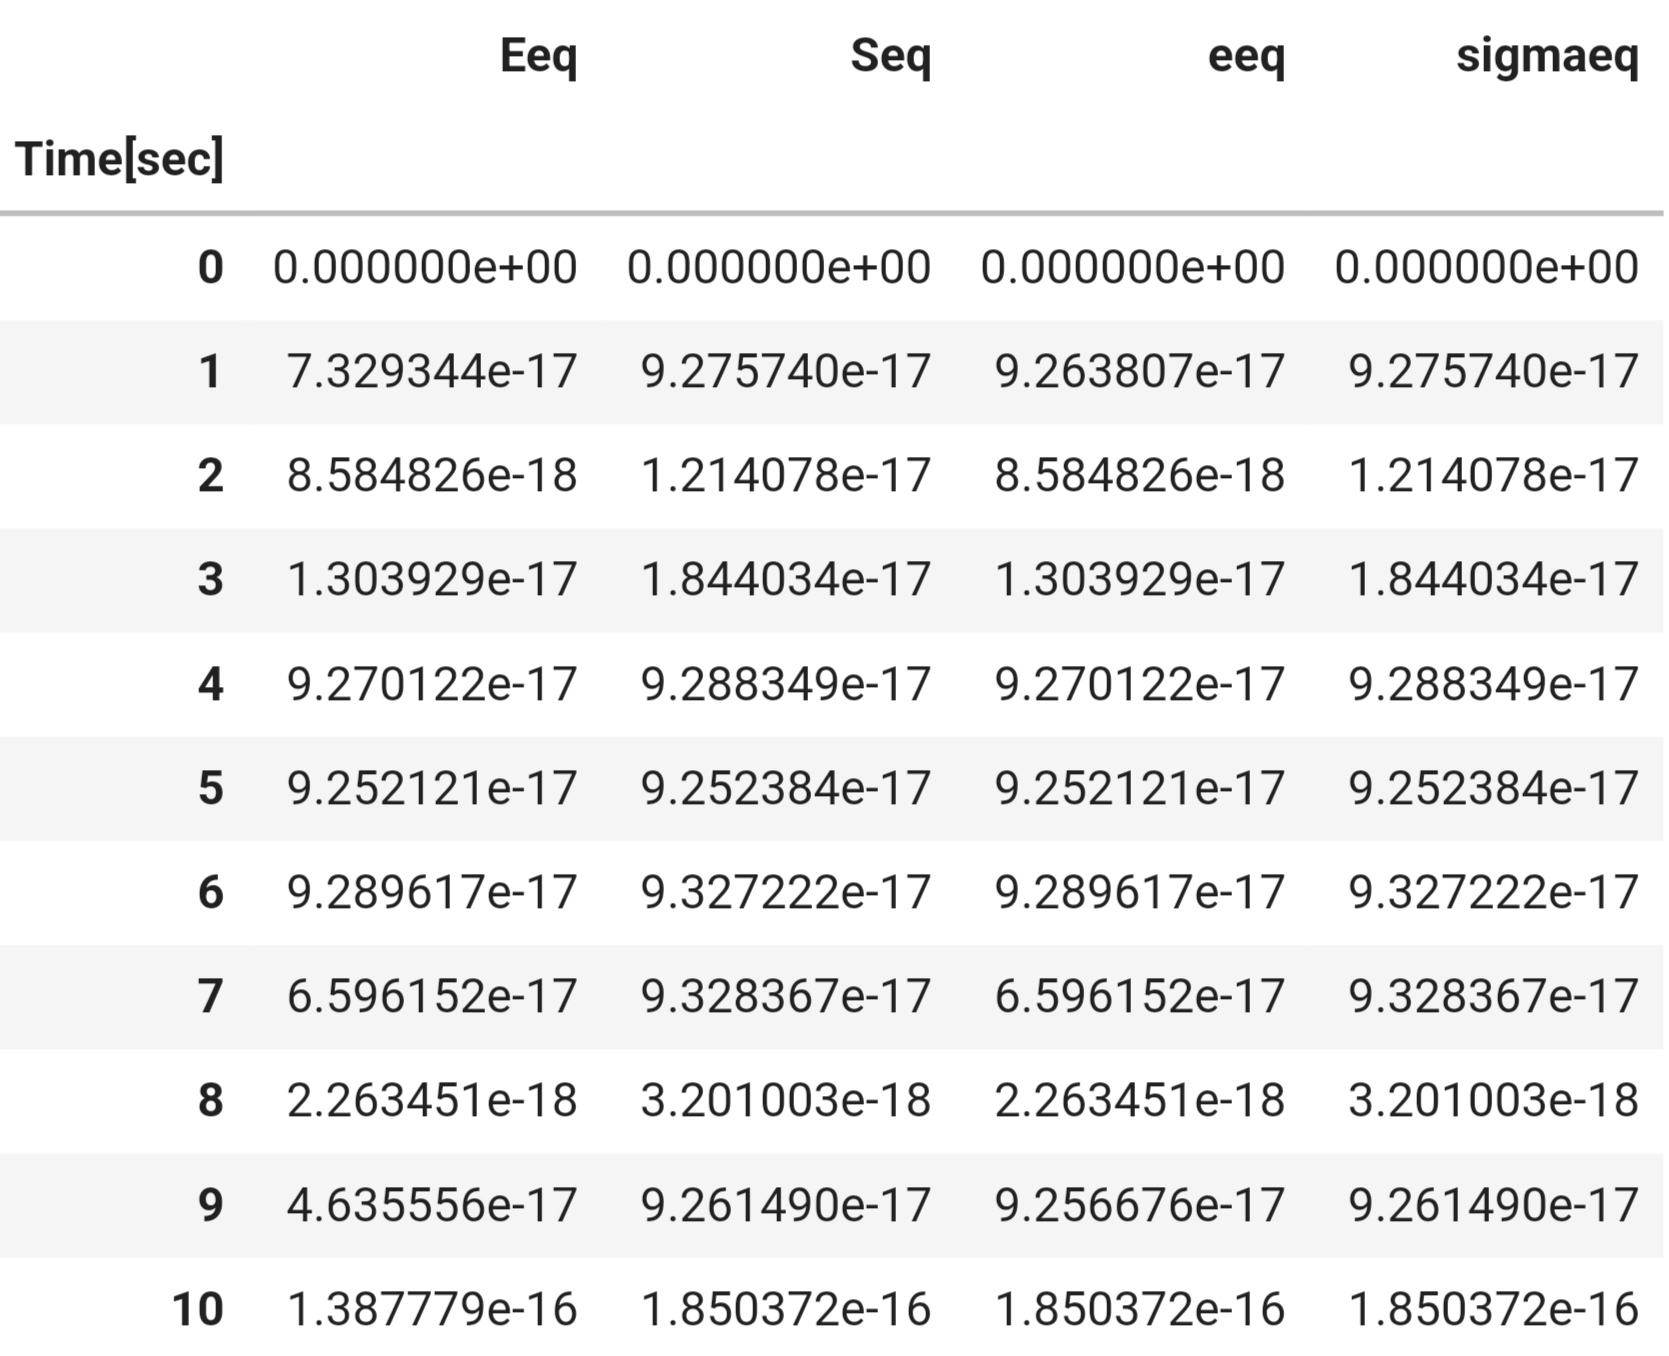
\includegraphics[width=\textwidth]{Values/m2t2.png}
        \end{block}
        \column[t]{0.48\textwidth}
        \begin{block}{\footnotesize Method-II(time integration)}
            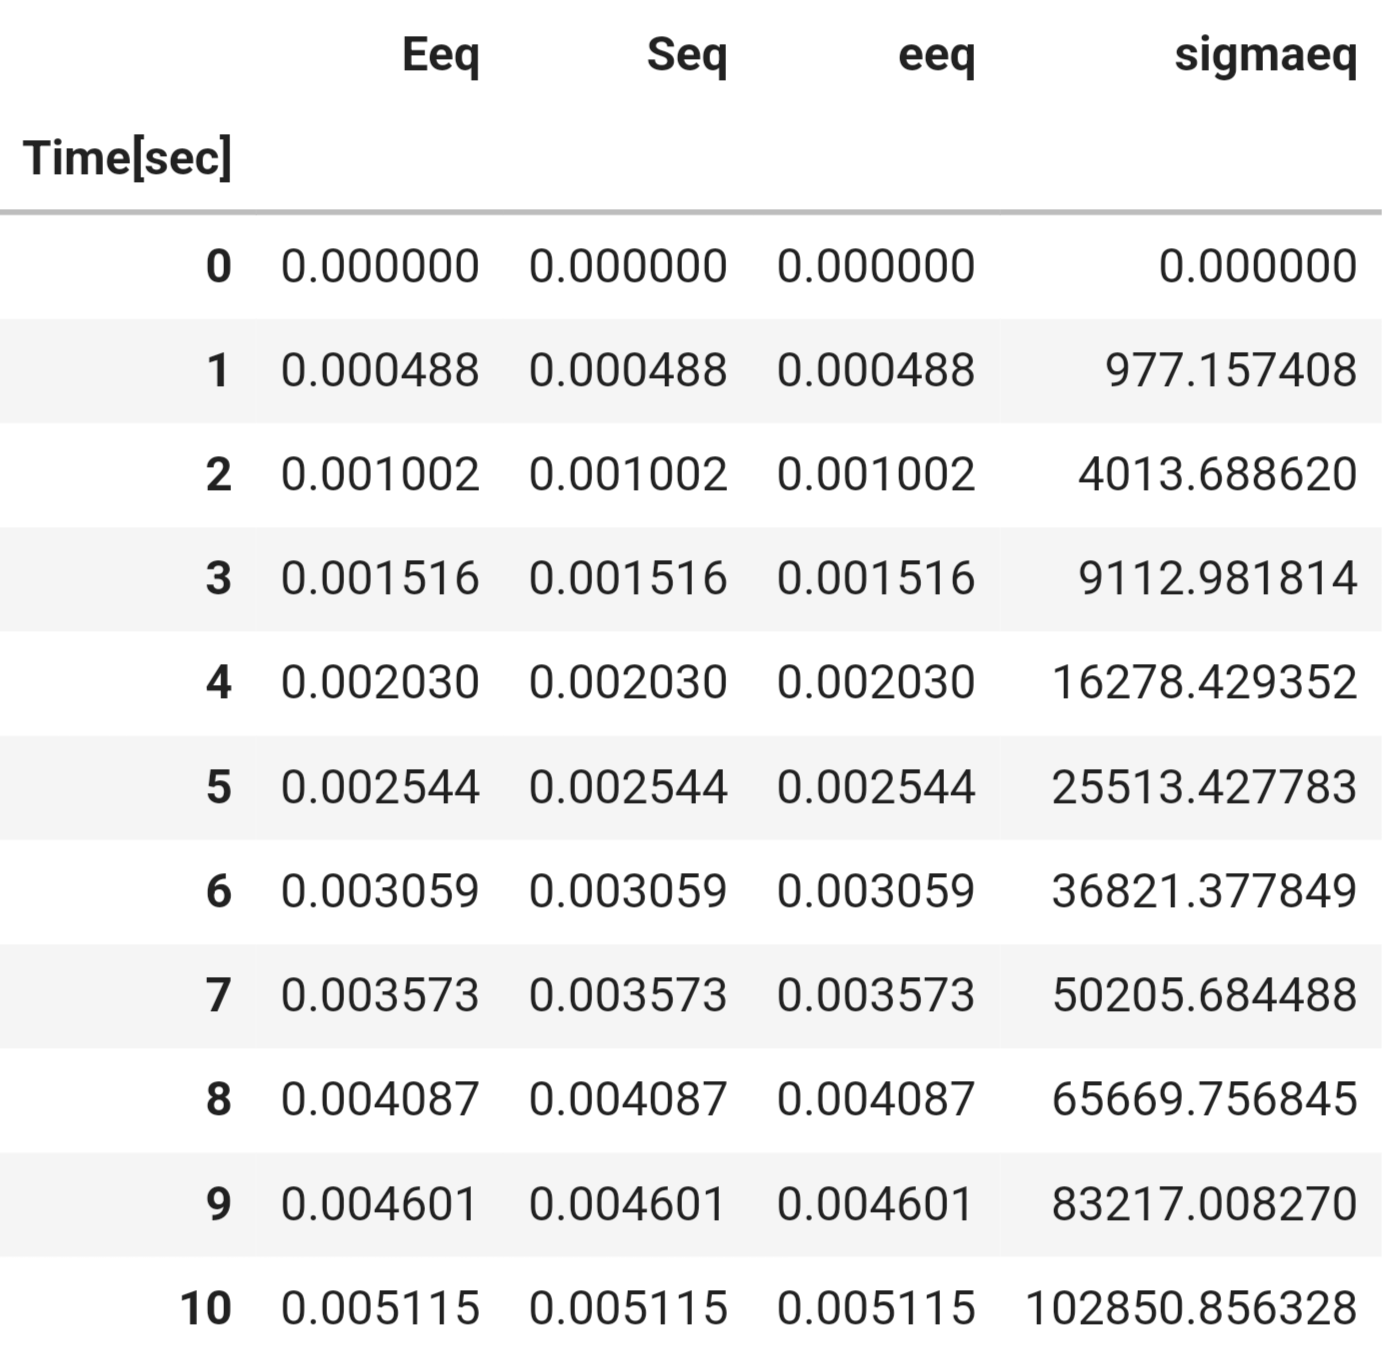
\includegraphics[width=\textwidth]{Values/m1t2.png}
        \end{block}
    \end{columns}
\end{frame}

%===================================================================
\section{Problem 3}

\begin{frame}{Problem 3 - Translation + Rotation}{Deformation and Stress vs Strain at t = 0 sec}
    \vspace{-2em}
    \scriptsize $$x_1 = X_1\cos\omega t - X_2\sin\omega t + t,\ x_2 = X_1\sin\omega t + X_2\cos\omega t + t,\ x_3 = X_3;\ \ \omega t = 90^o \implies \omega = 9^o$$
    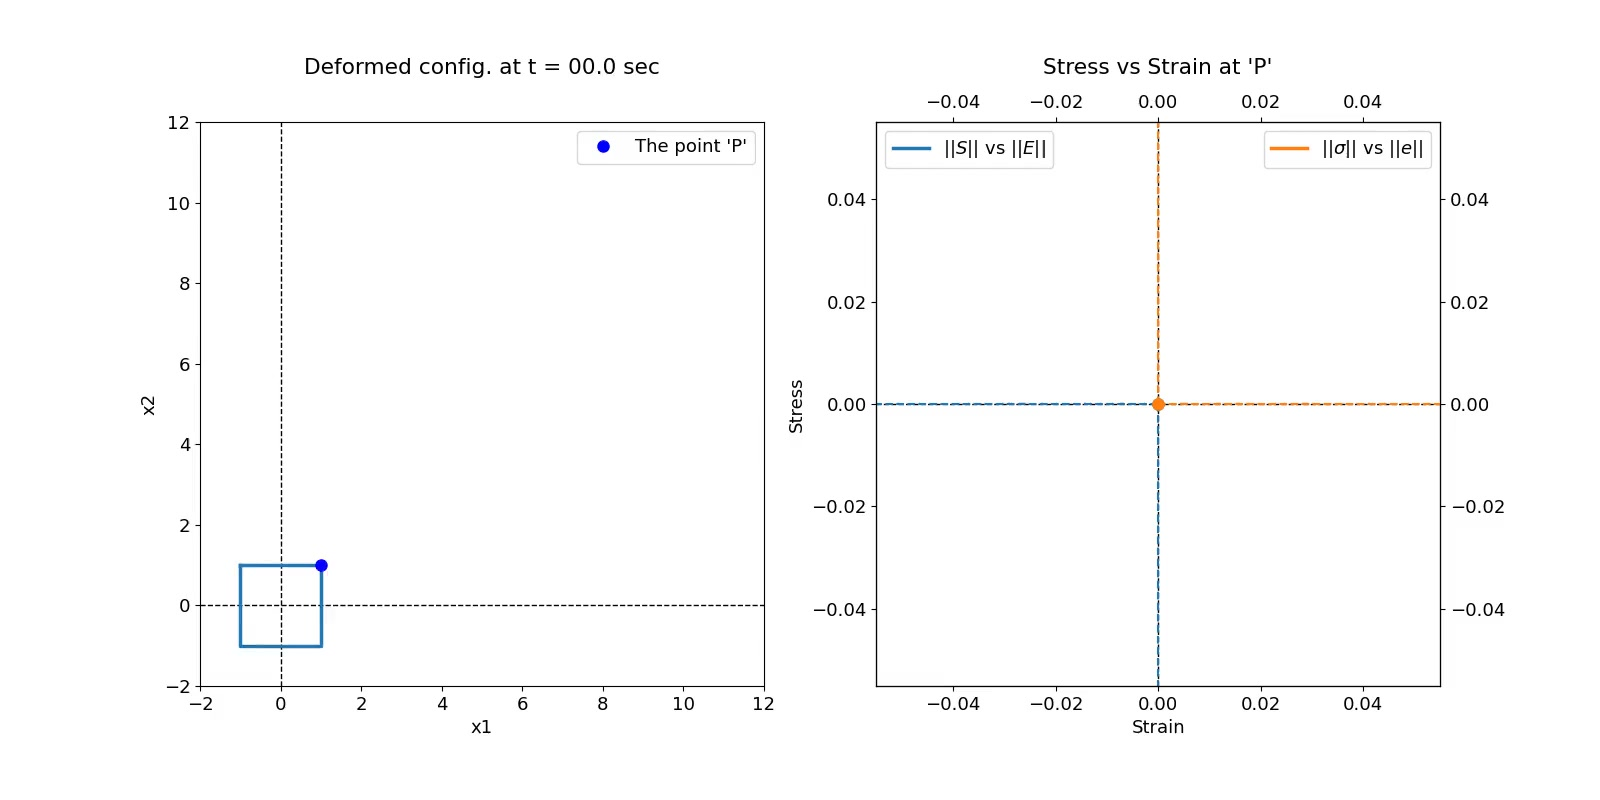
\includegraphics[width=\textwidth, trim={4.5cm 2cm 3cm 1cm}, clip]{Plots/itrandrotation.jpg}
\end{frame}

\begin{frame}{Problem 3 - Translation + Rotation}{Deformation and Stress vs Strain at t = 10 sec}
    \vspace{-2em}
    \scriptsize $$x_1 = X_1\cos\omega t - X_2\sin\omega t + t,\ x_2 = X_1\sin\omega t + X_2\cos\omega t + t,\ x_3 = X_3;\ \ \omega t = 90^o \implies \omega = 9^o$$
    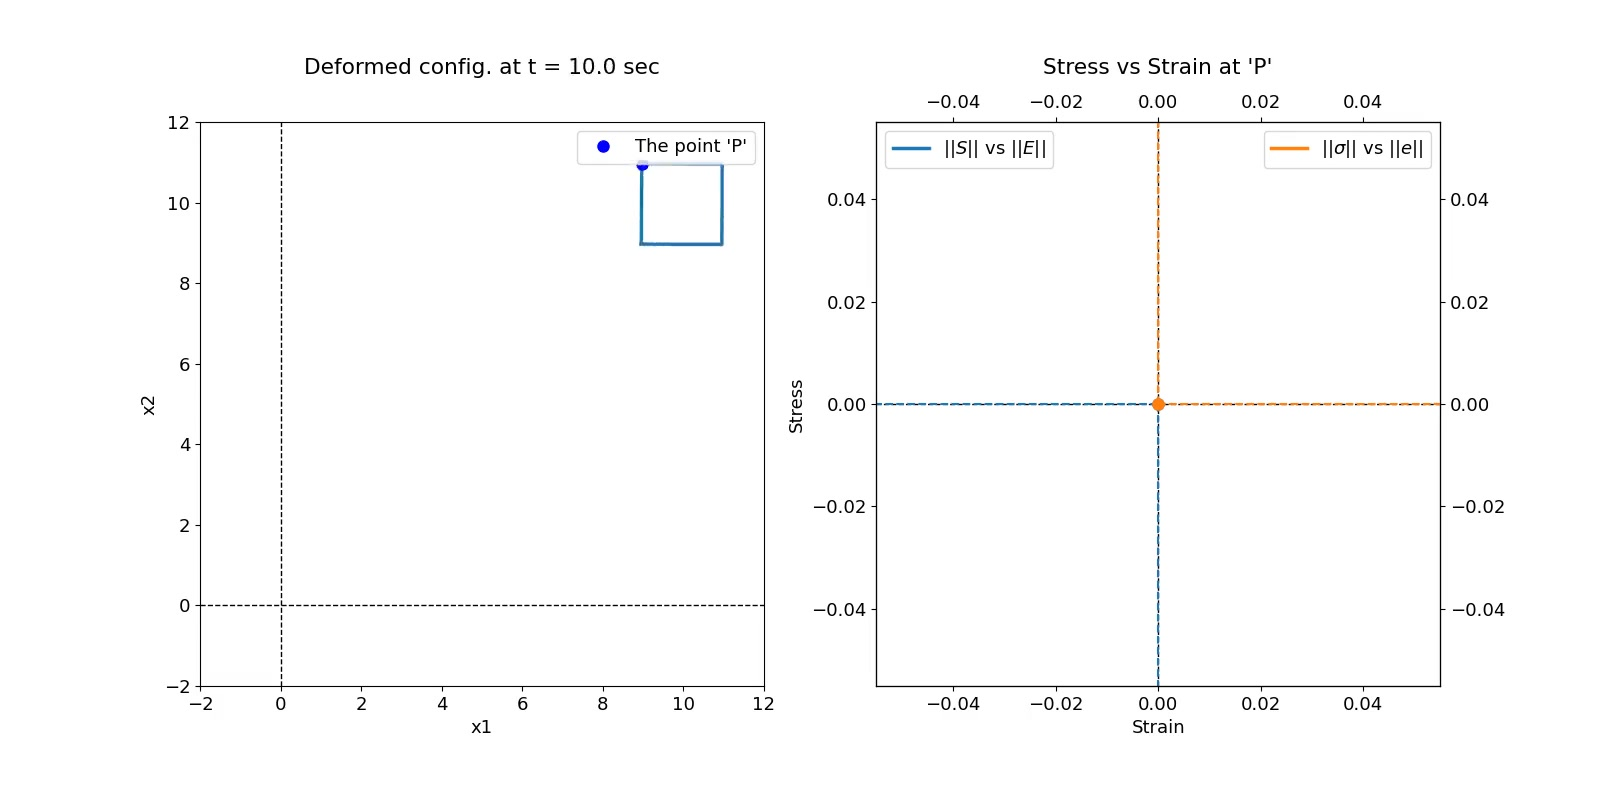
\includegraphics[width=\textwidth, trim={4.5cm 2cm 3cm 1cm}, clip]{Plots/trandrotation.jpg}
\end{frame}

\begin{frame}{Problem 3 - Translation + Rotation}{Method-I vs Method-II(time integration)}
    \vspace{-2em}
    \begin{columns}
        \column[t]{0.48\textwidth}
        \begin{block}{\footnotesize Method-I}
            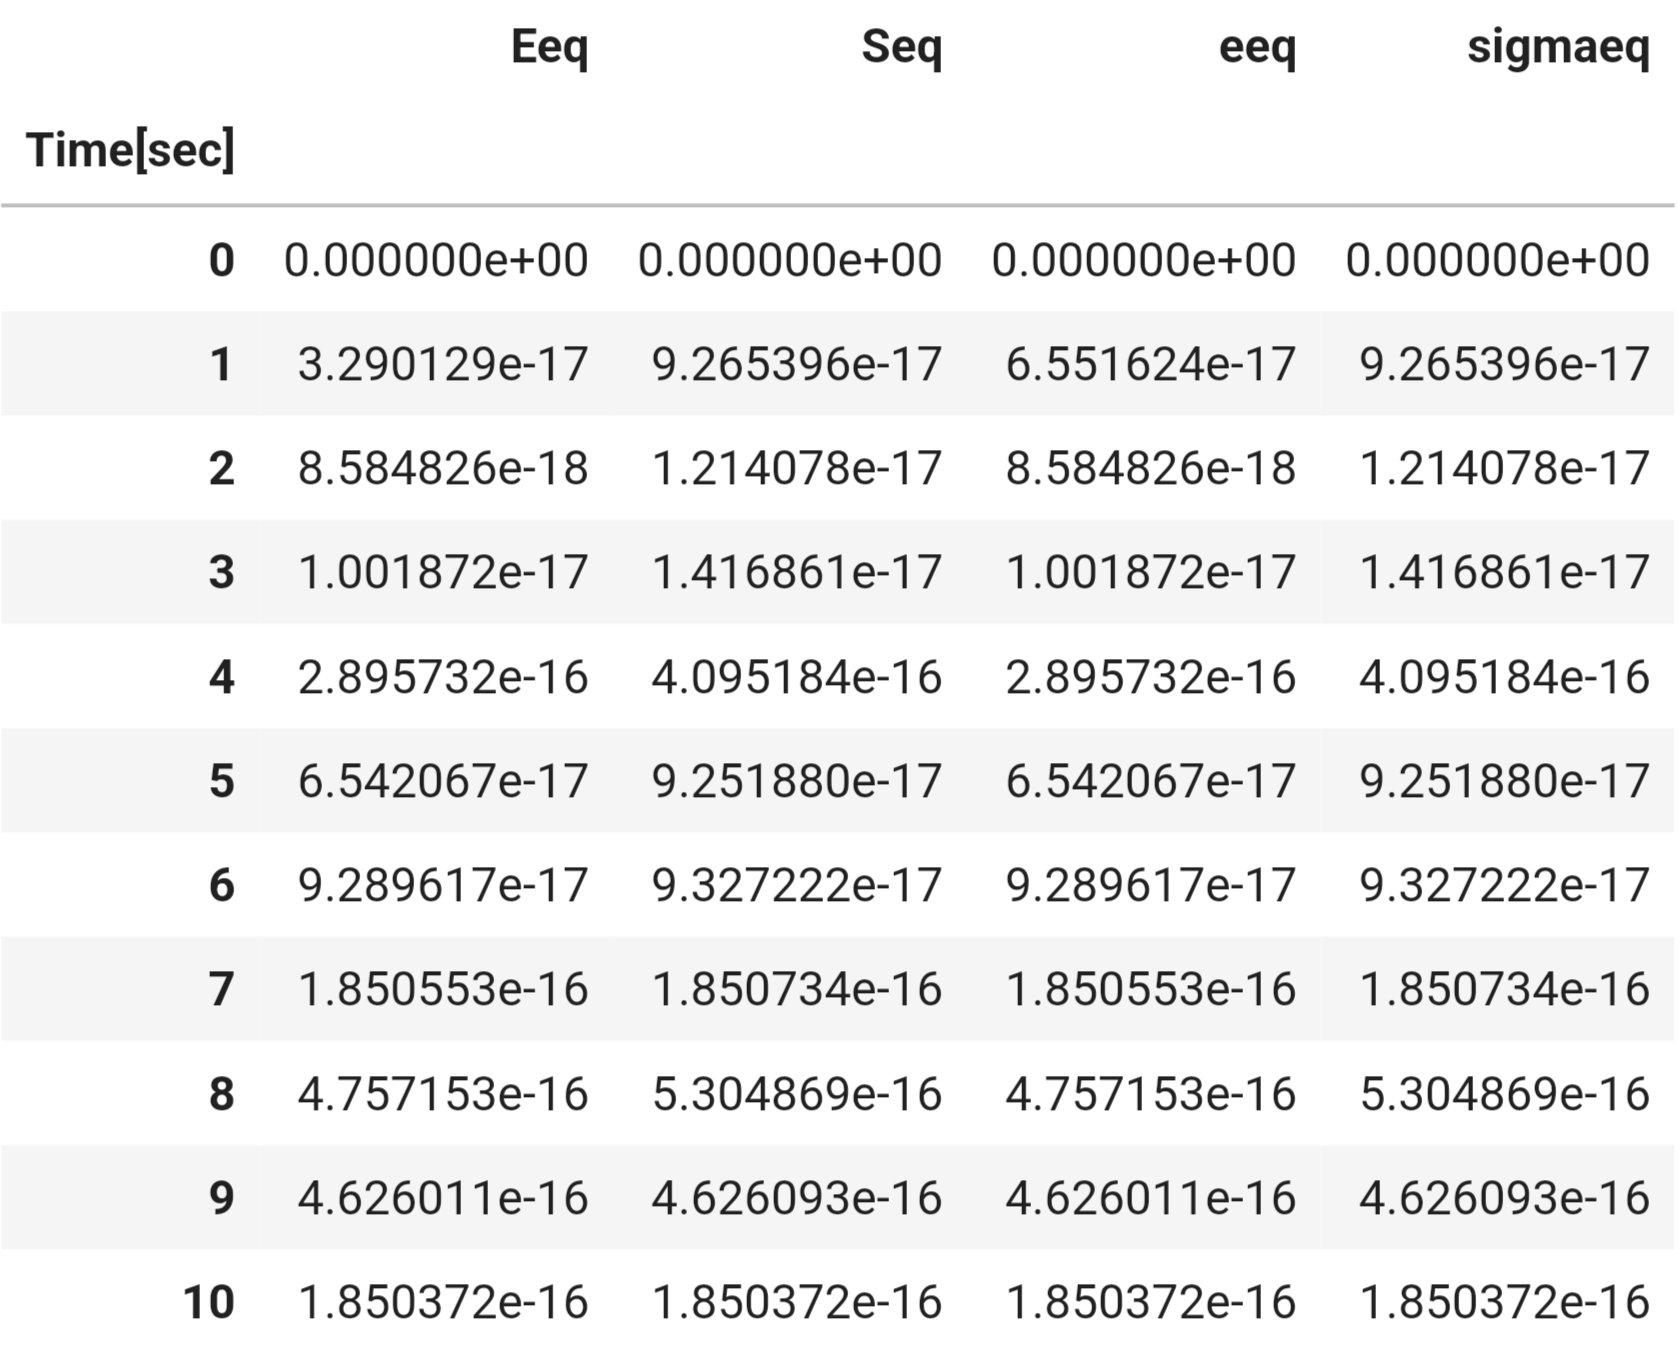
\includegraphics[width=\textwidth]{Values/m2t3.png}
        \end{block}
        \column[t]{0.48\textwidth}
        \begin{block}{\footnotesize Method-II(time integration)}
            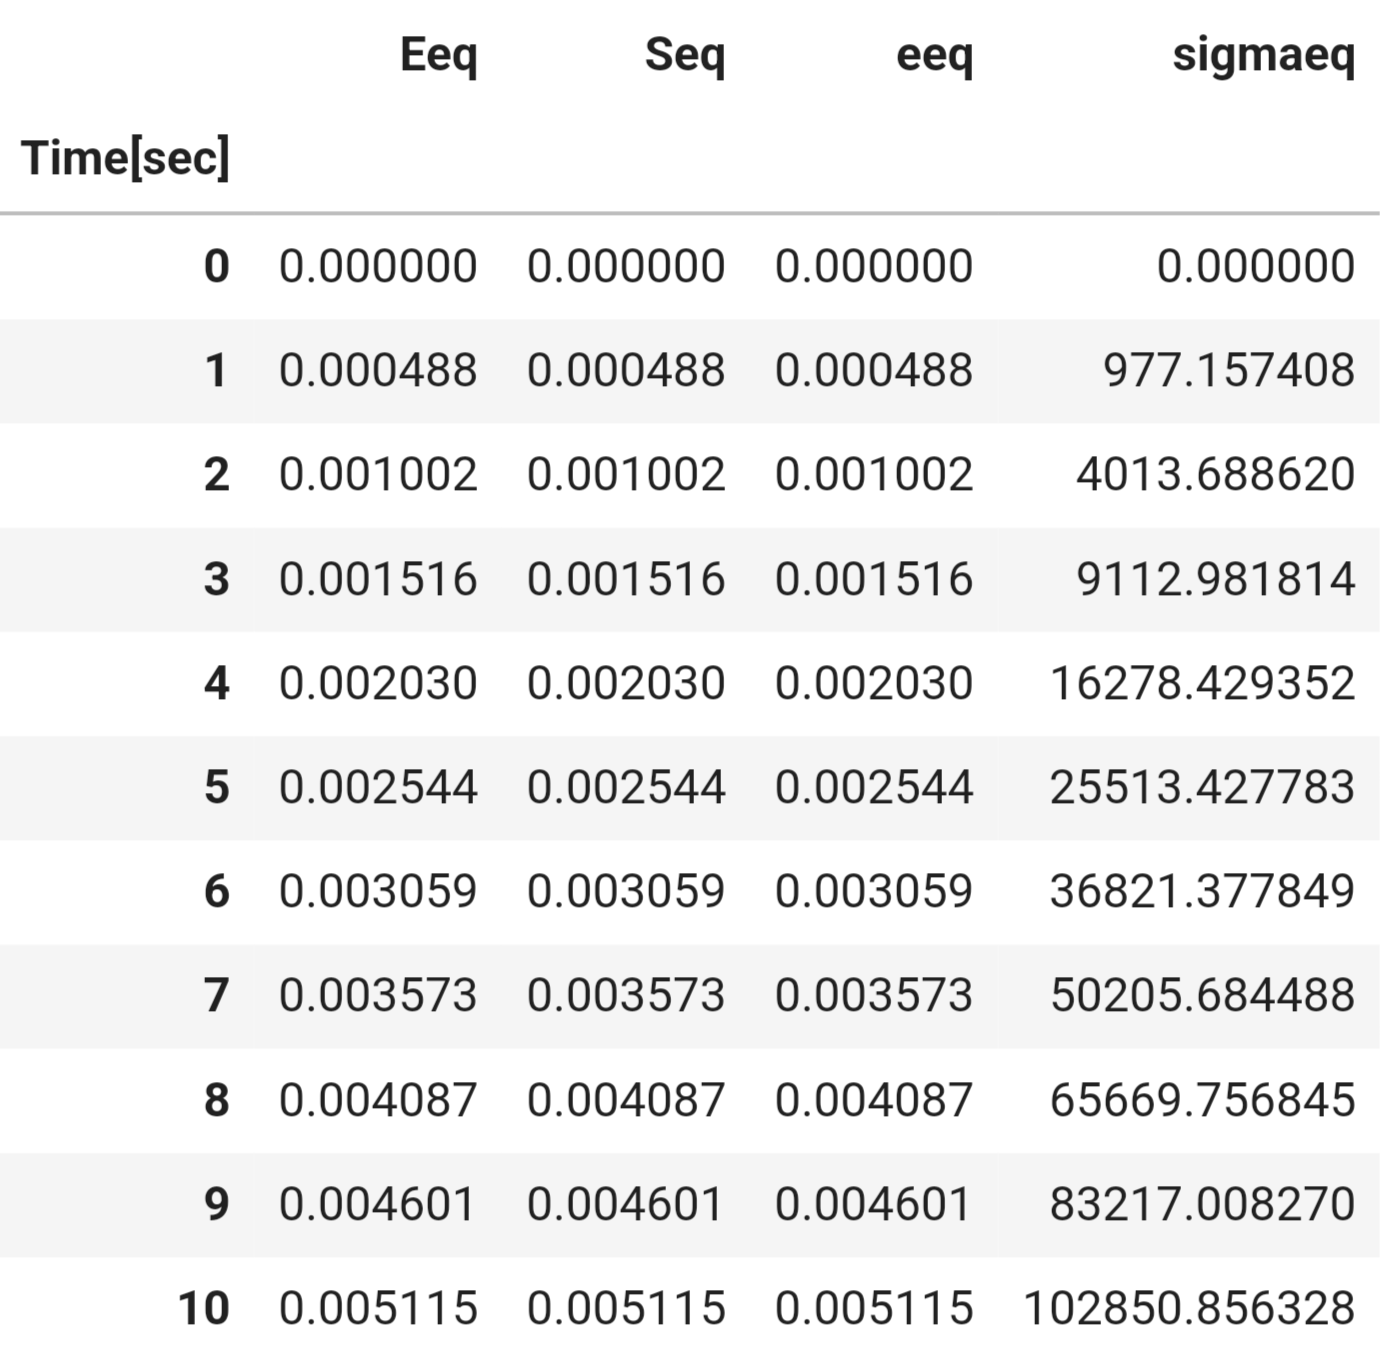
\includegraphics[width=\textwidth]{Values/m1t3.png}
        \end{block}
    \end{columns}
\end{frame}

%===================================================================
\section{Problem 4}

\begin{frame}{Problem 4 - Pure Shear}{Deformation and Stress vs Strain at t = 0 sec}
    \vspace{-1em}
    \scriptsize $$x_1 = X_1 + X_2t,\ x_2 = X_2,\ x_3 = X_3$$
    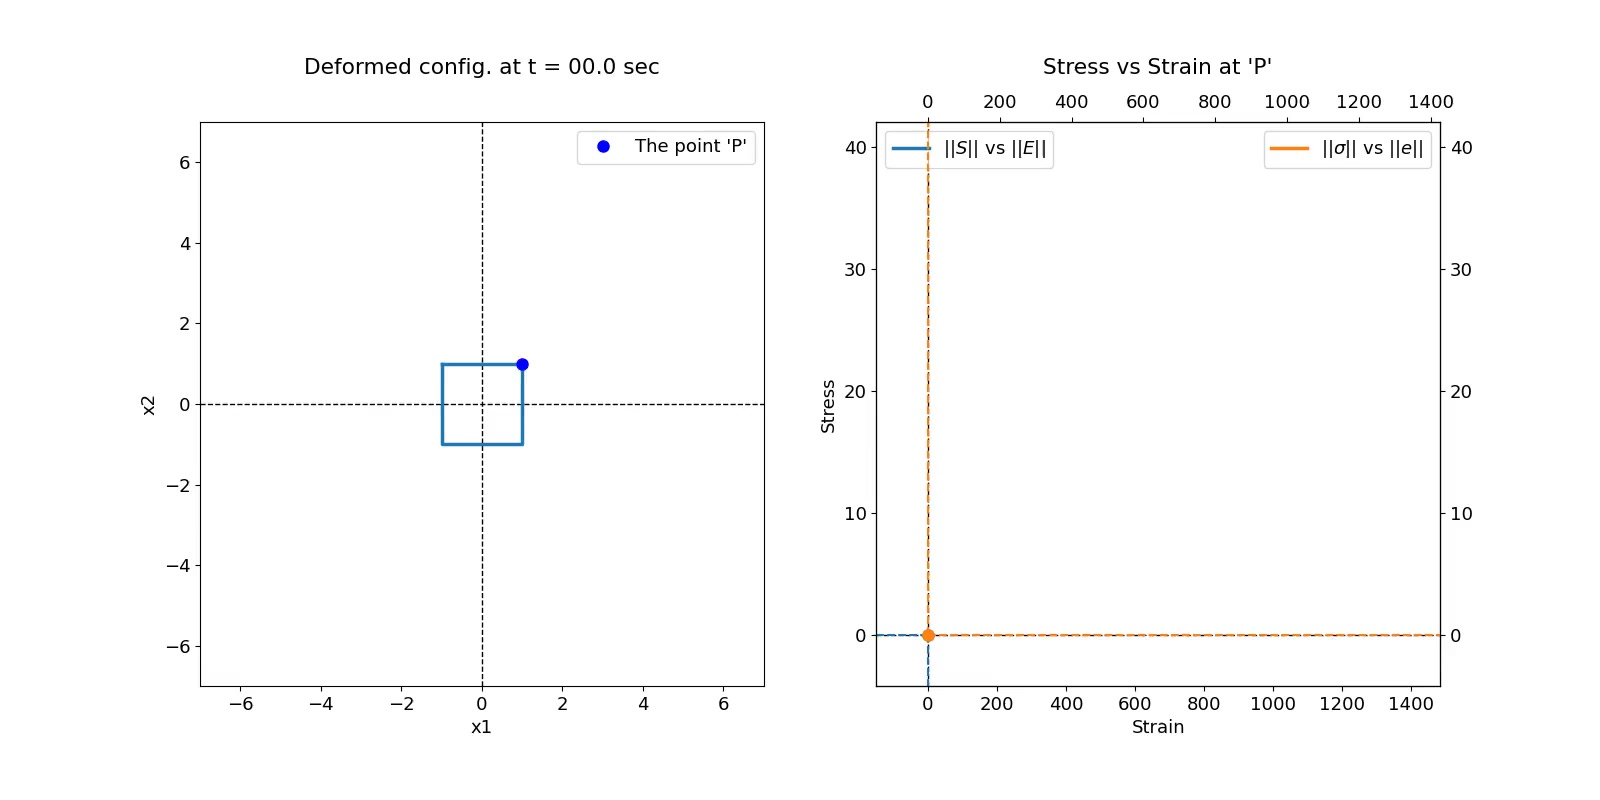
\includegraphics[width=\textwidth, trim={4.5cm 2cm 3cm 1cm}, clip]{Plots/ipureshear.jpg}
\end{frame}

\begin{frame}{Problem 4 - Pure Shear}{Deformation and Stress vs Strain at t = 10 sec}
    \vspace{-1em}
    \scriptsize $$x_1 = X_1 + X_2t,\ x_2 = X_2,\ x_3 = X_3$$
    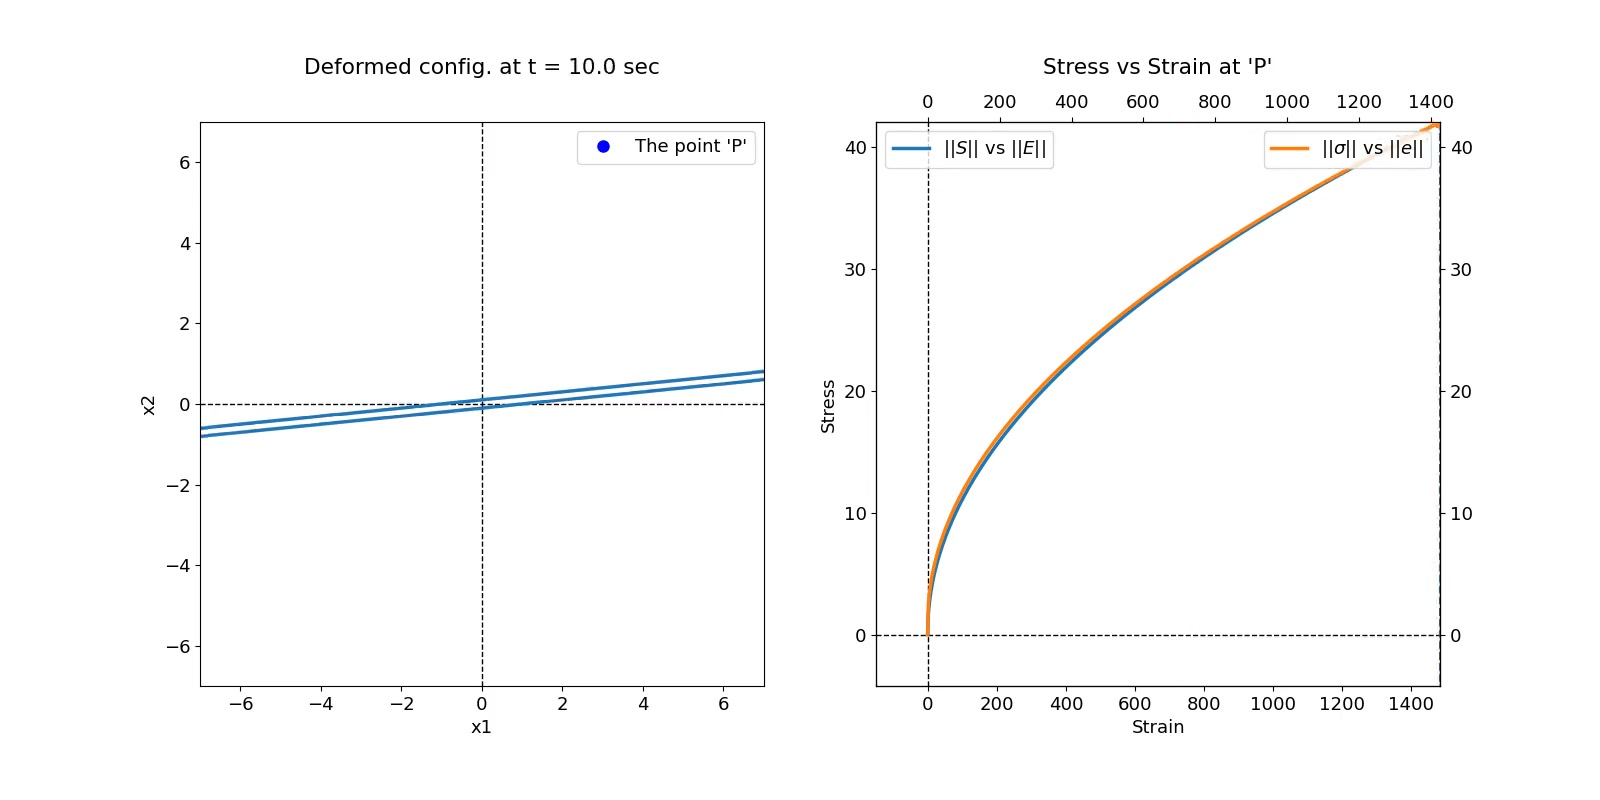
\includegraphics[width=\textwidth, trim={4.5cm 2cm 3cm 1cm}, clip]{Plots/pureshear.jpg}
\end{frame}

\begin{frame}{Problem 4 - Pure Shear}{Method-I vs Method-II(time integration)}
    \vspace{-2em}
    \begin{columns}
        \column[t]{0.48\textwidth}
        \begin{block}{\footnotesize Method-I}
            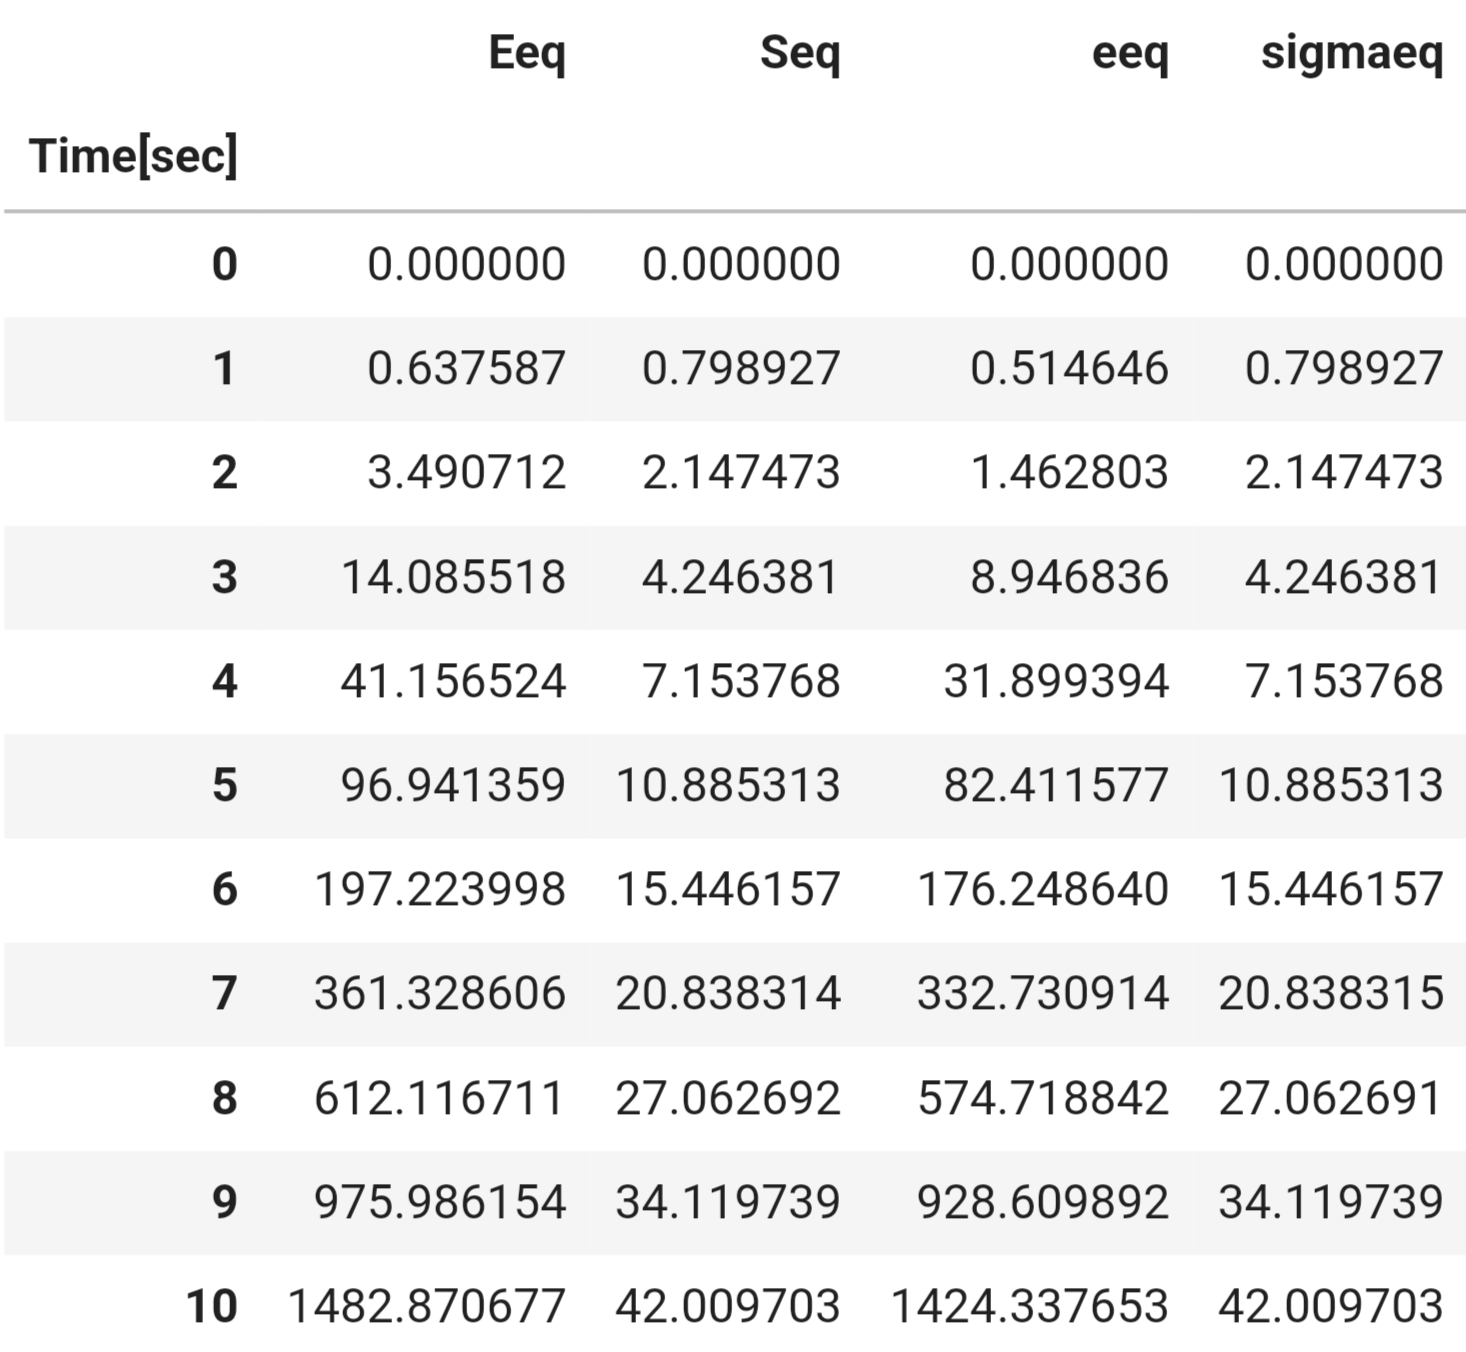
\includegraphics[width=\textwidth]{Values/m2t4.png}
        \end{block}
        \column[t]{0.48\textwidth}
        \begin{block}{\footnotesize Method-II(time integration)}
            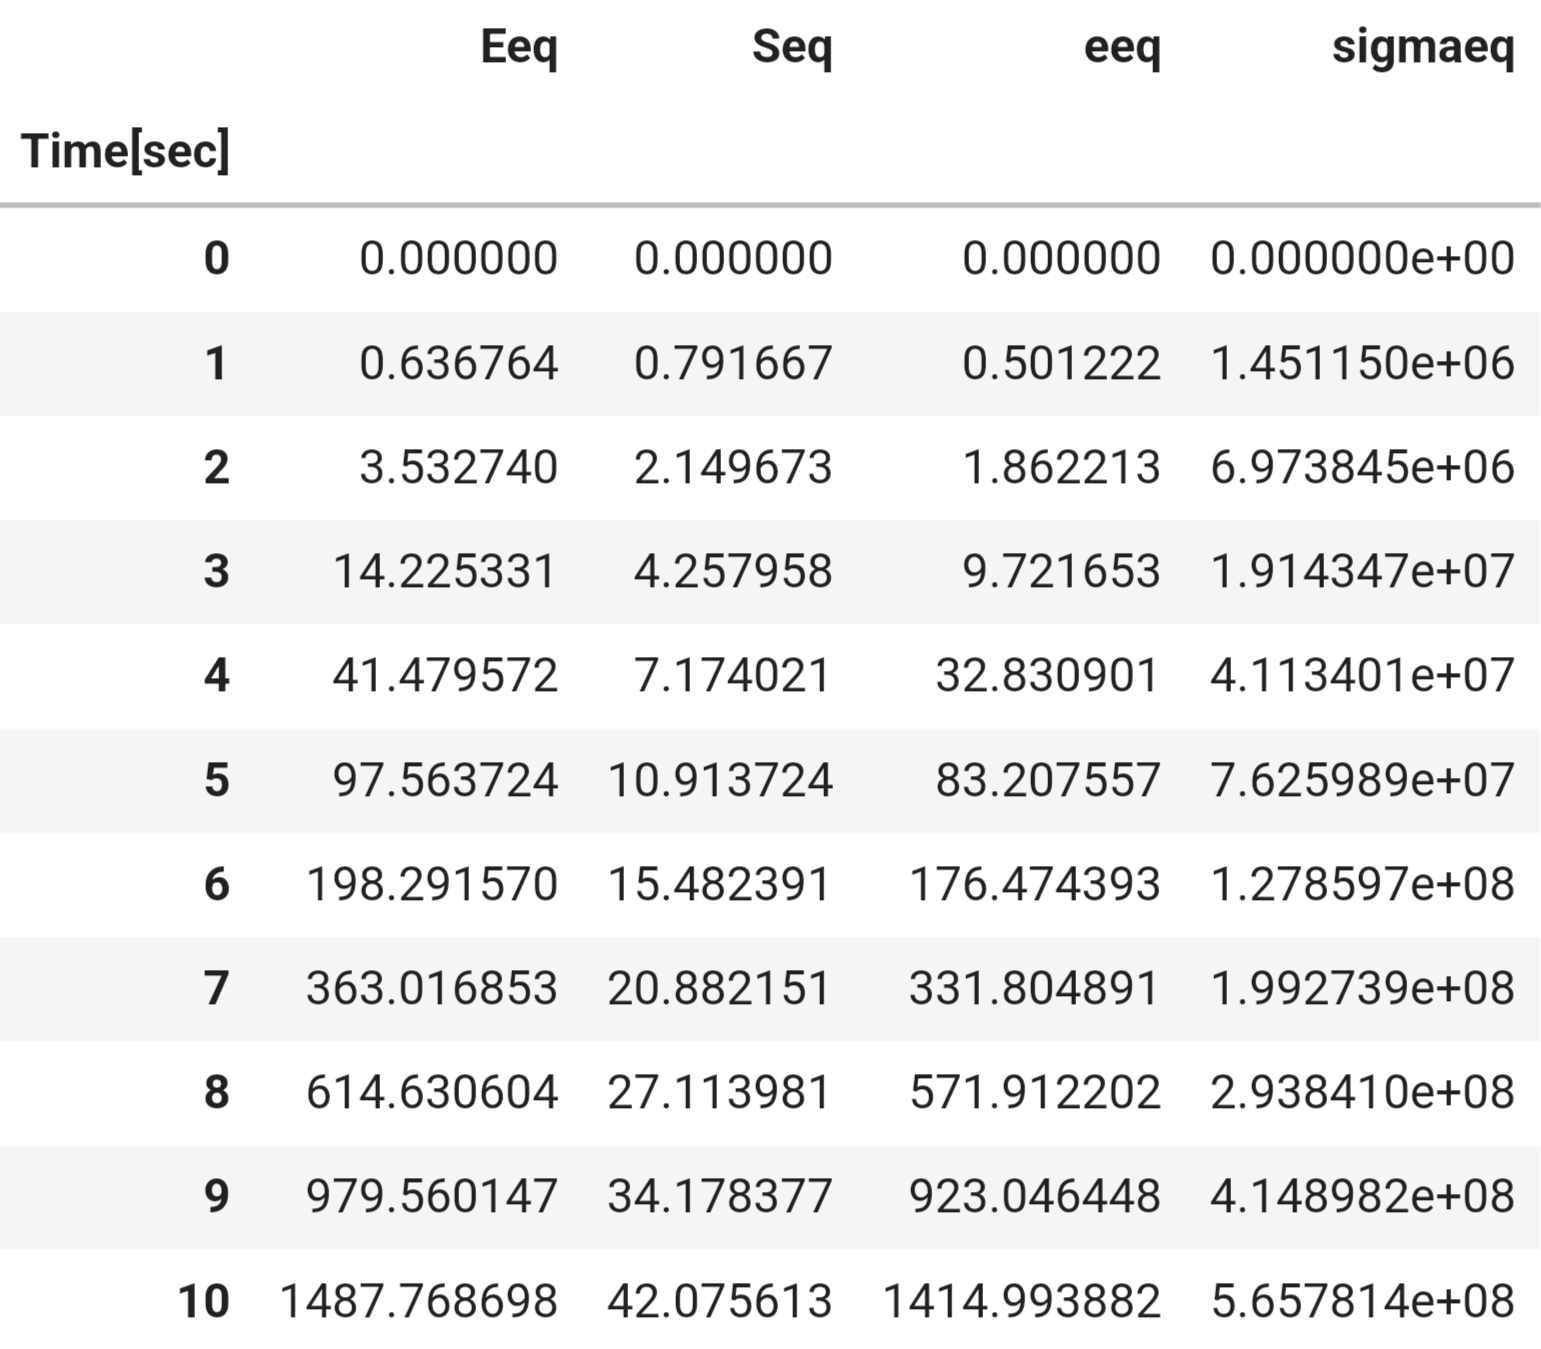
\includegraphics[width=\textwidth]{Values/m1t4.png}
        \end{block}
    \end{columns}
\end{frame}

%===================================================================
\section{Problem 5}

\begin{frame}{Problem 5 - Generic}{Deformation and Stress vs Strain at t = 0 sec}
    \vspace{-1em}
    \scriptsize $$x_1 = X_1e^t + X_3(e^t-1),\ x_2 = X_2 + X_3(e^t-e^{-t}),\ x_3 = X_3$$
    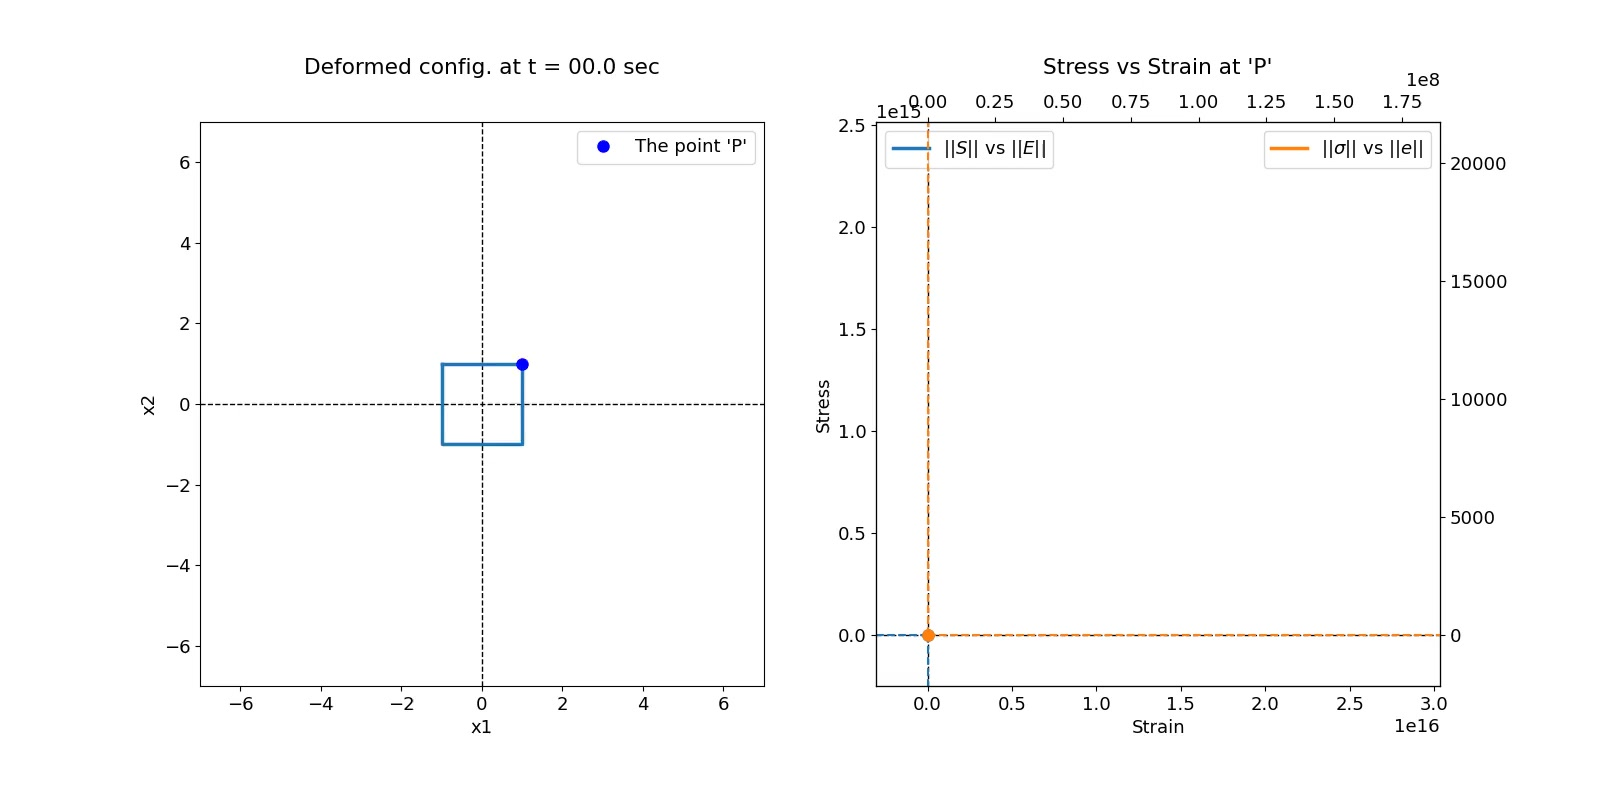
\includegraphics[width=\textwidth, trim={4.5cm 2cm 3cm 1cm}, clip]{Plots/igeneric.jpg}
\end{frame}

\begin{frame}{Problem 5 - Generic}{Deformation and Stress vs Strain at t = 10 sec}
    \vspace{-1em}
    \scriptsize $$x_1 = X_1e^t + X_3(e^t-1),\ x_2 = X_2 + X_3(e^t-e^{-t}),\ x_3 = X_3$$
    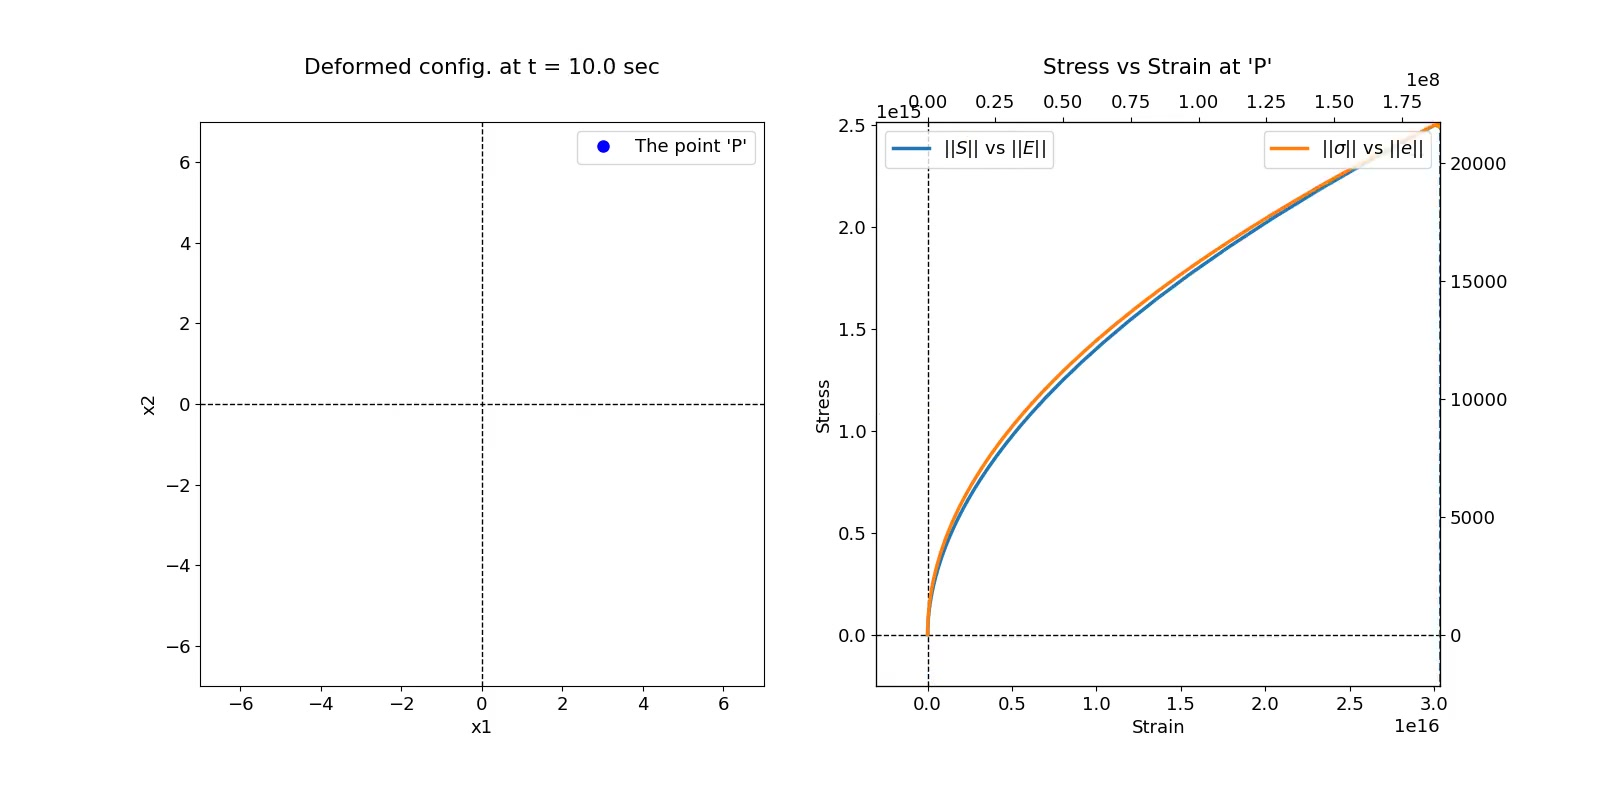
\includegraphics[width=\textwidth, trim={4.5cm 2cm 3cm 1cm}, clip]{Plots/generic.jpg}
\end{frame}

\begin{frame}{Problem 5 - Generic}{Method-I vs Method-II(time integration)}
    \vspace{-2em}
    \begin{columns}
        \column[t]{0.48\textwidth}
        \begin{block}{\footnotesize Method-I}
            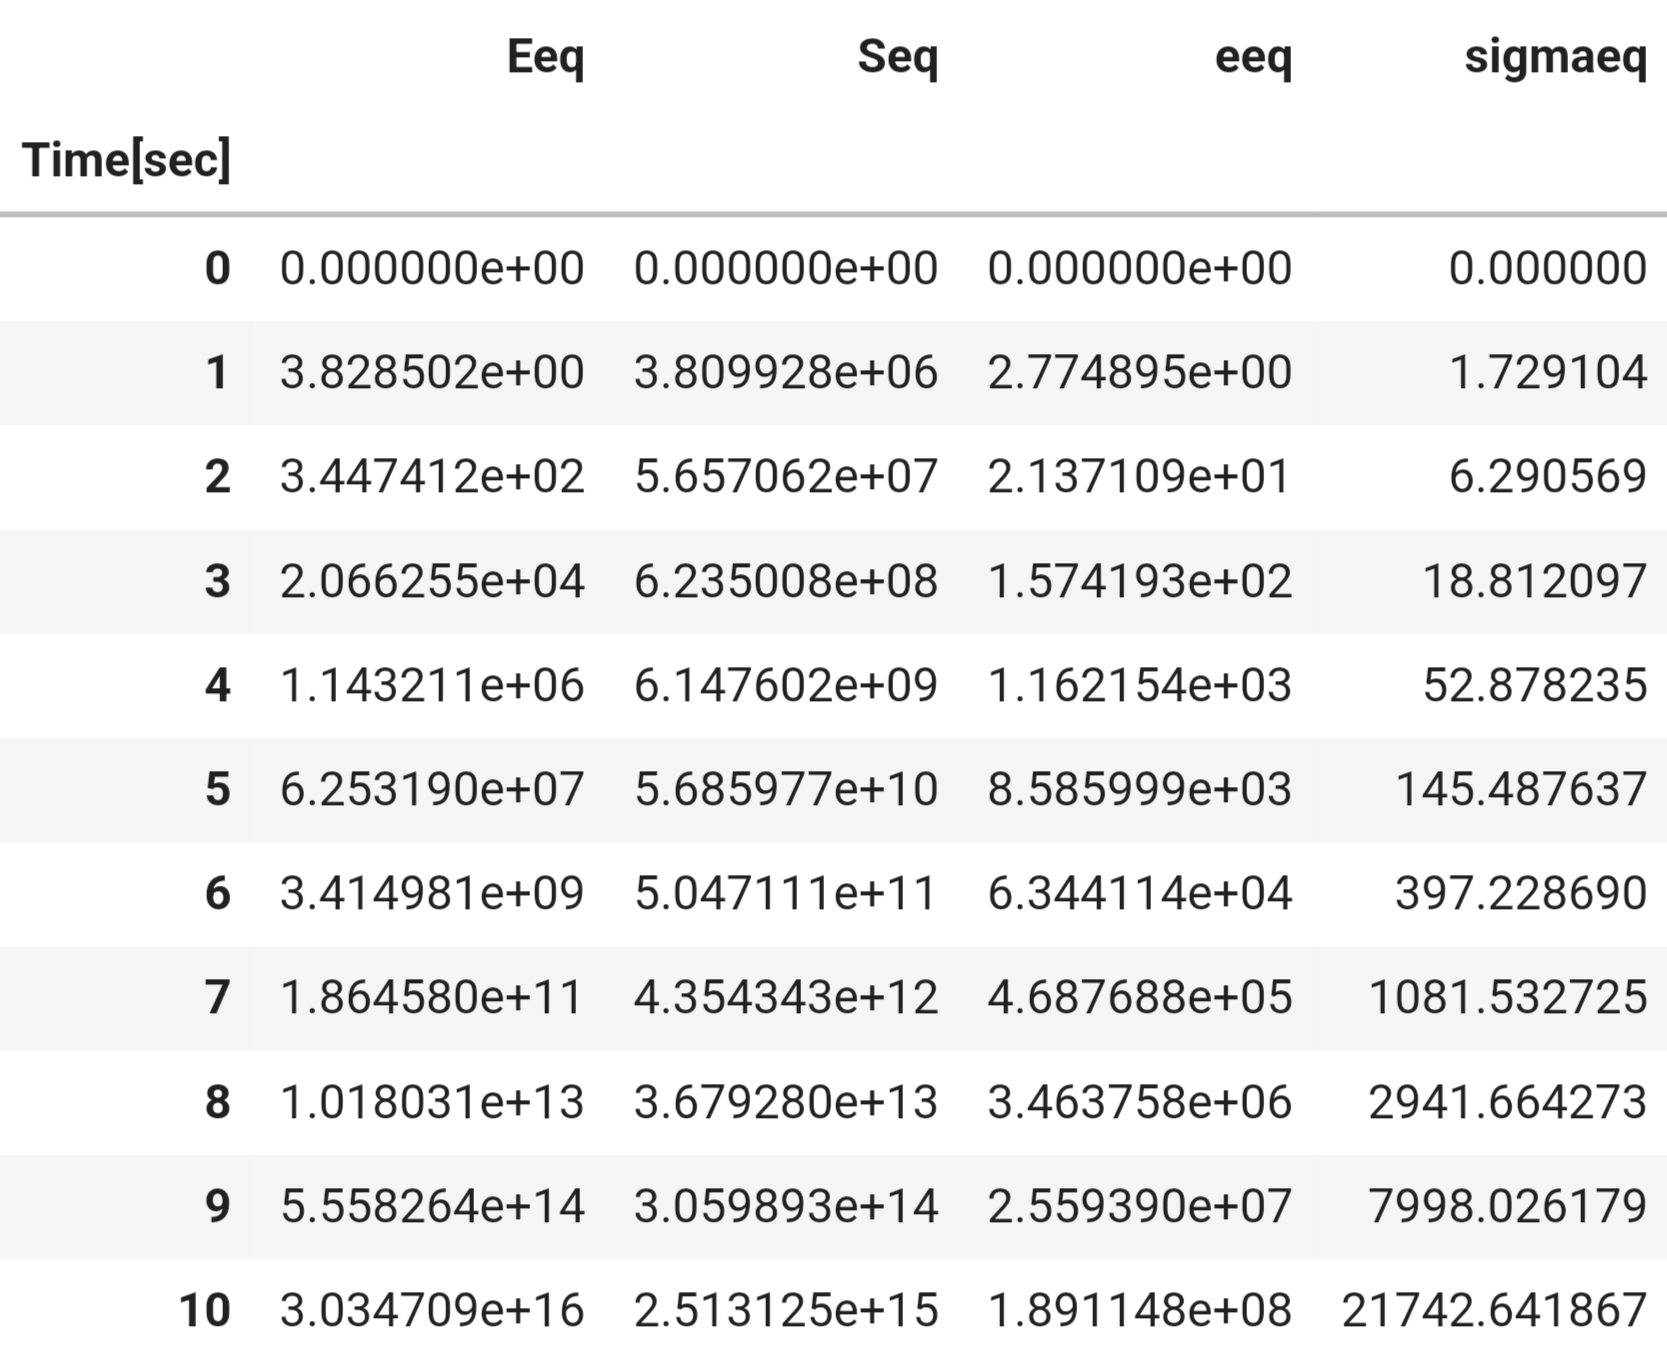
\includegraphics[width=\textwidth]{Values/m2t5.png}
        \end{block}
        \column[t]{0.48\textwidth}
        \begin{block}{\footnotesize Method-II(time integration)}
            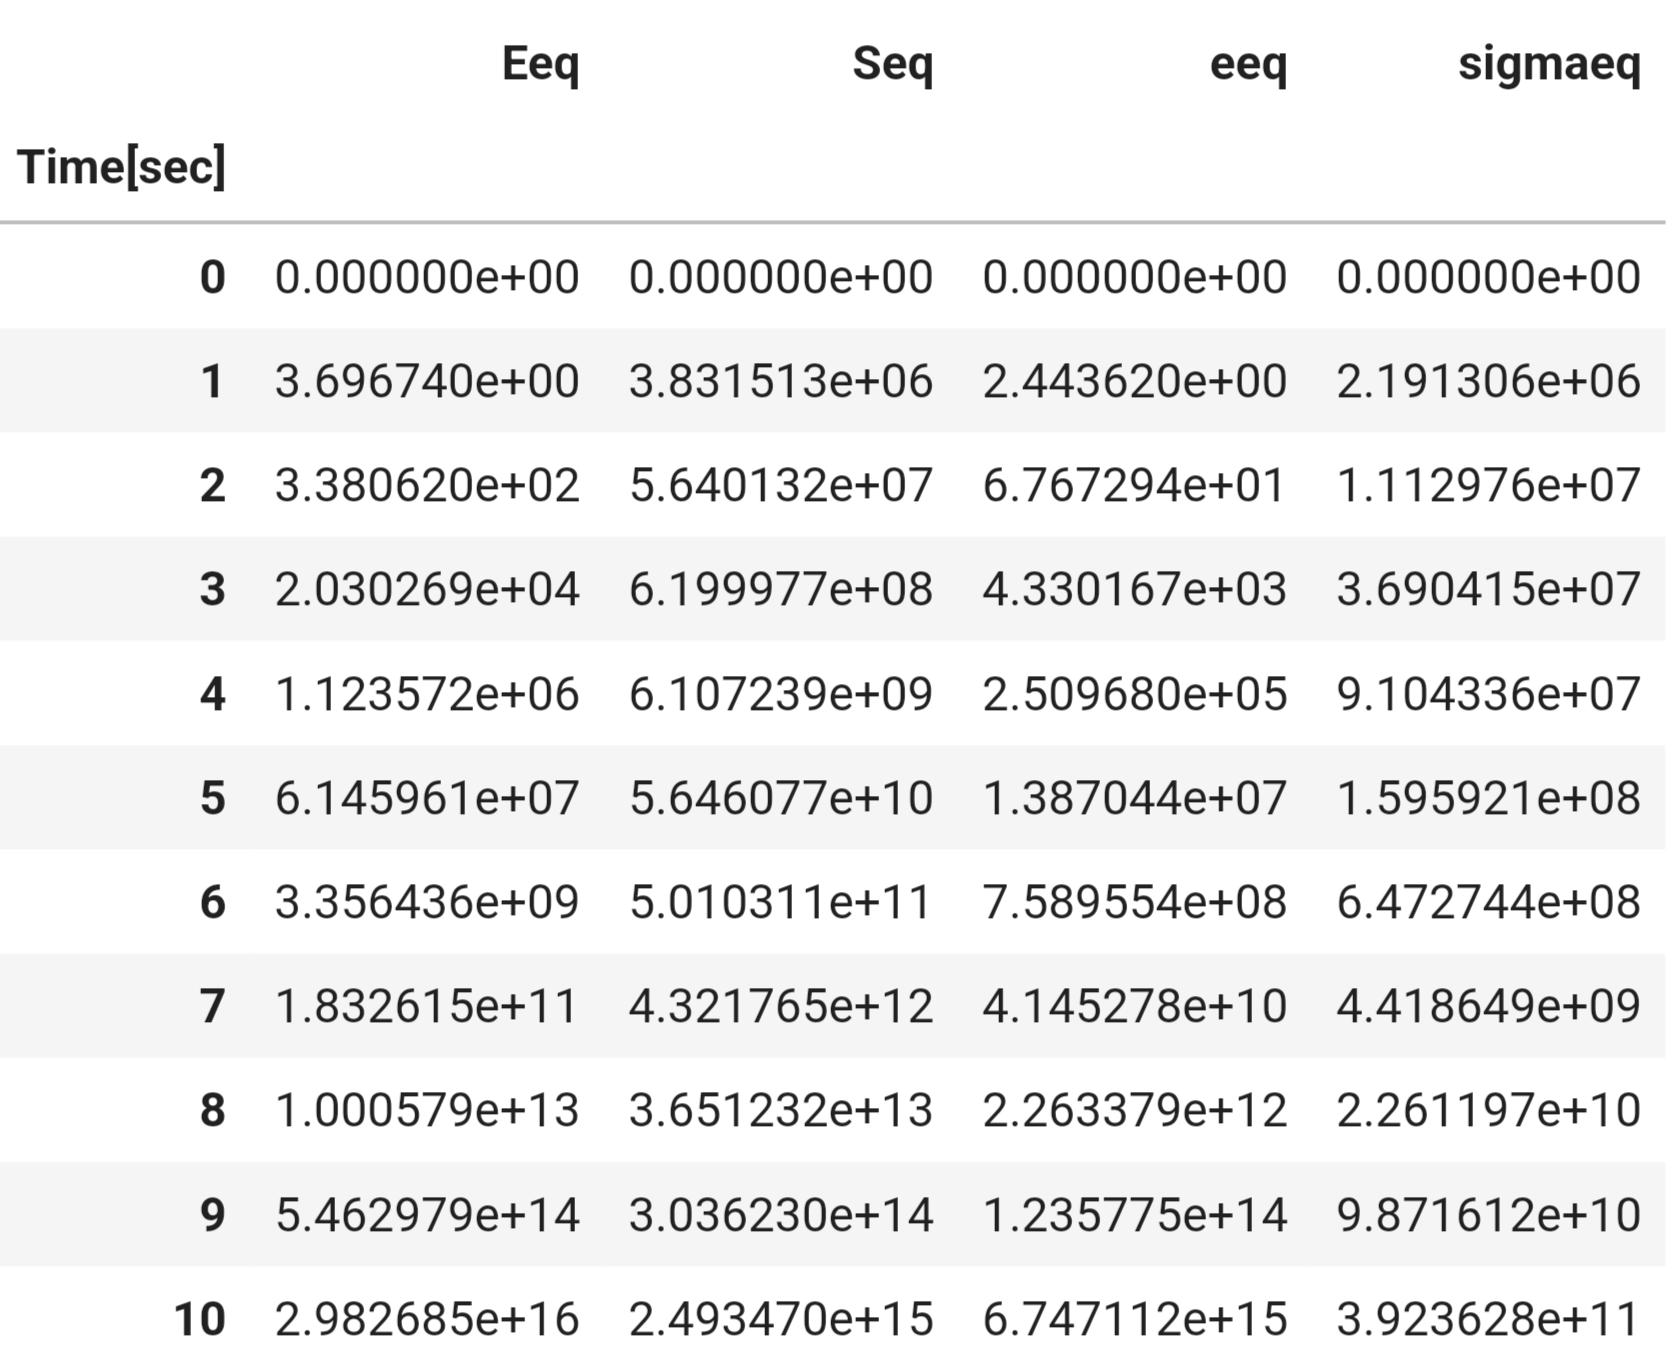
\includegraphics[width=\textwidth]{Values/m1t5.png}
        \end{block}
    \end{columns}
\end{frame}

%===================================================================
\section{Problem 6}

\begin{frame}{Problem 6 - Biaxial Tension}{Deformation and Stress vs Strain at t = 0 sec}
    \vspace{-1em}
    \scriptsize $$x_1 = X_1 + X_1t,\ x_2 = X_2 + X_2t,\ x_3 = X_3$$
    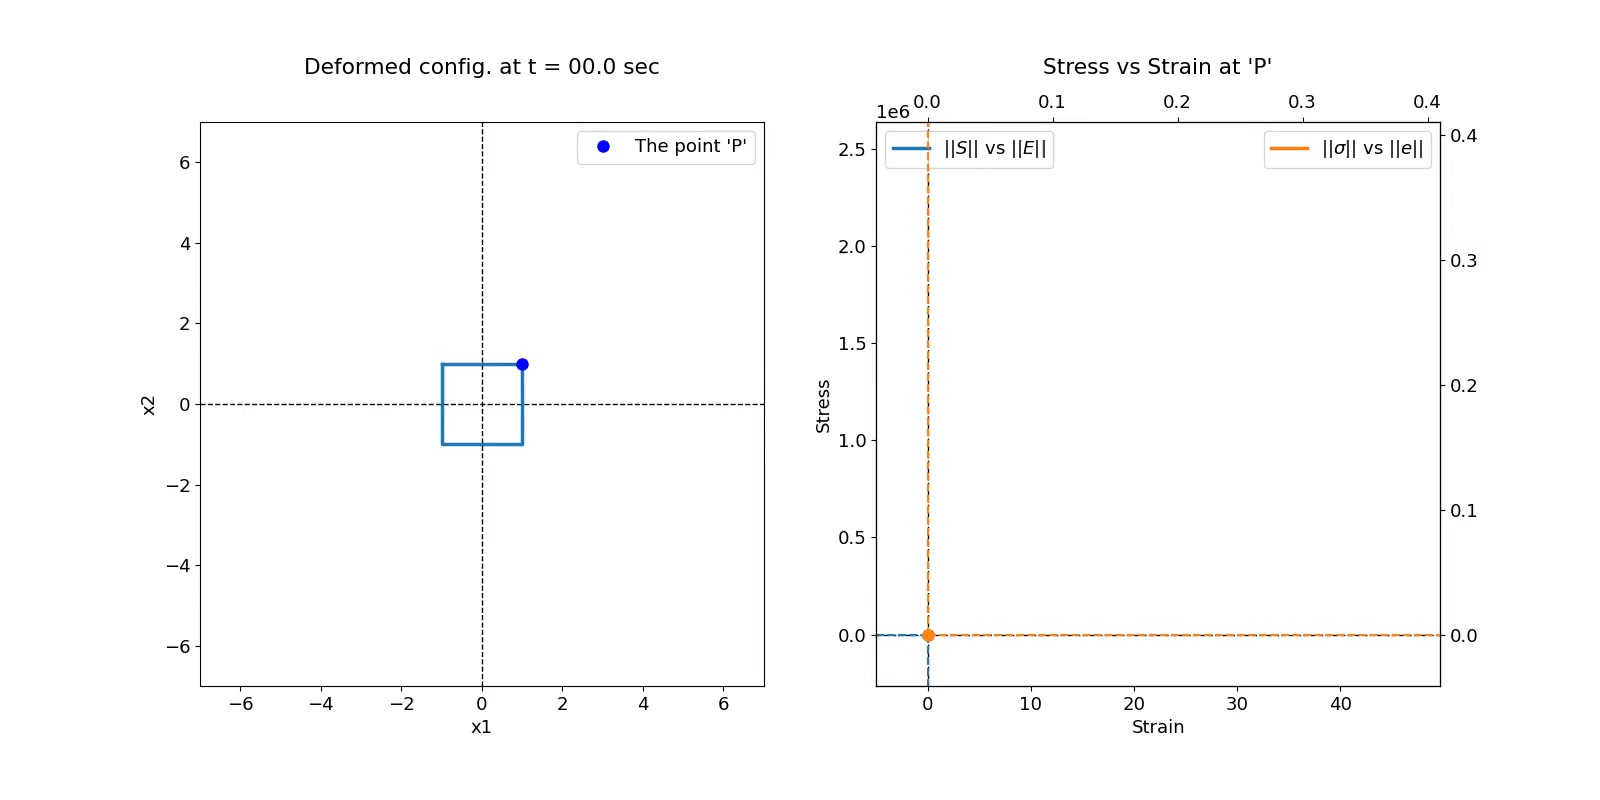
\includegraphics[width=\textwidth, trim={4.5cm 2cm 3cm 1cm}, clip]{Plots/ibitension.jpg}
\end{frame}

\begin{frame}{Problem 6 - Biaxial Tension}{Deformation and Stress vs Strain at t = 10 sec}
    \vspace{-1em}
    \scriptsize $$x_1 = X_1 + X_1t,\ x_2 = X_2 + X_2t,\ x_3 = X_3$$
    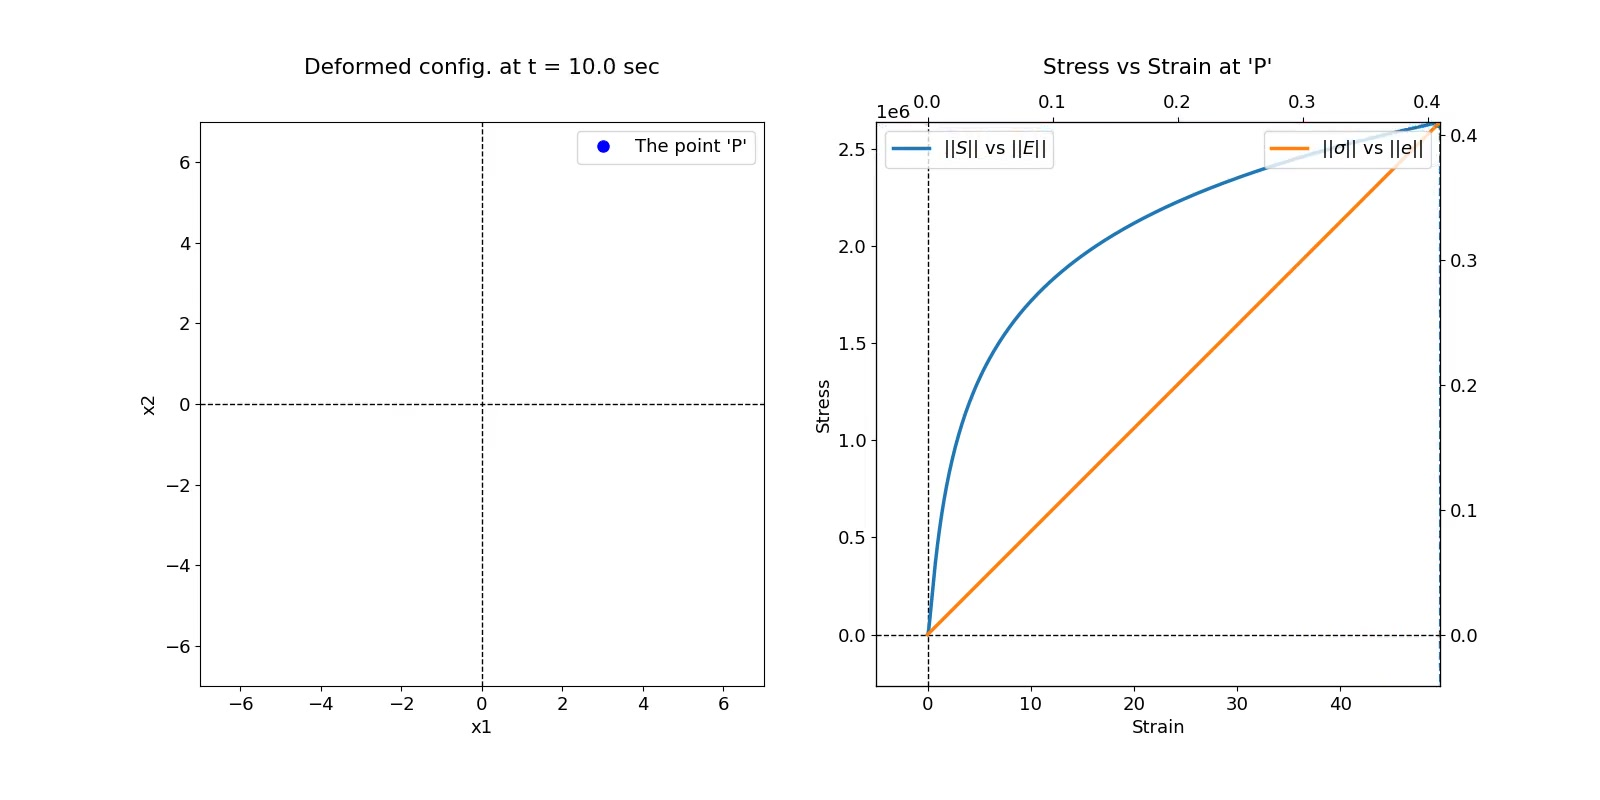
\includegraphics[width=\textwidth, trim={4.5cm 2cm 3cm 1cm}, clip]{Plots/bitension.jpg}
\end{frame}

\begin{frame}{Problem 6 - Biaxial Tension}{Method-I vs Method-II(time integration)}
    \vspace{-2em}
    \begin{columns}
        \column[t]{0.48\textwidth}
        \begin{block}{\footnotesize Method-I}
            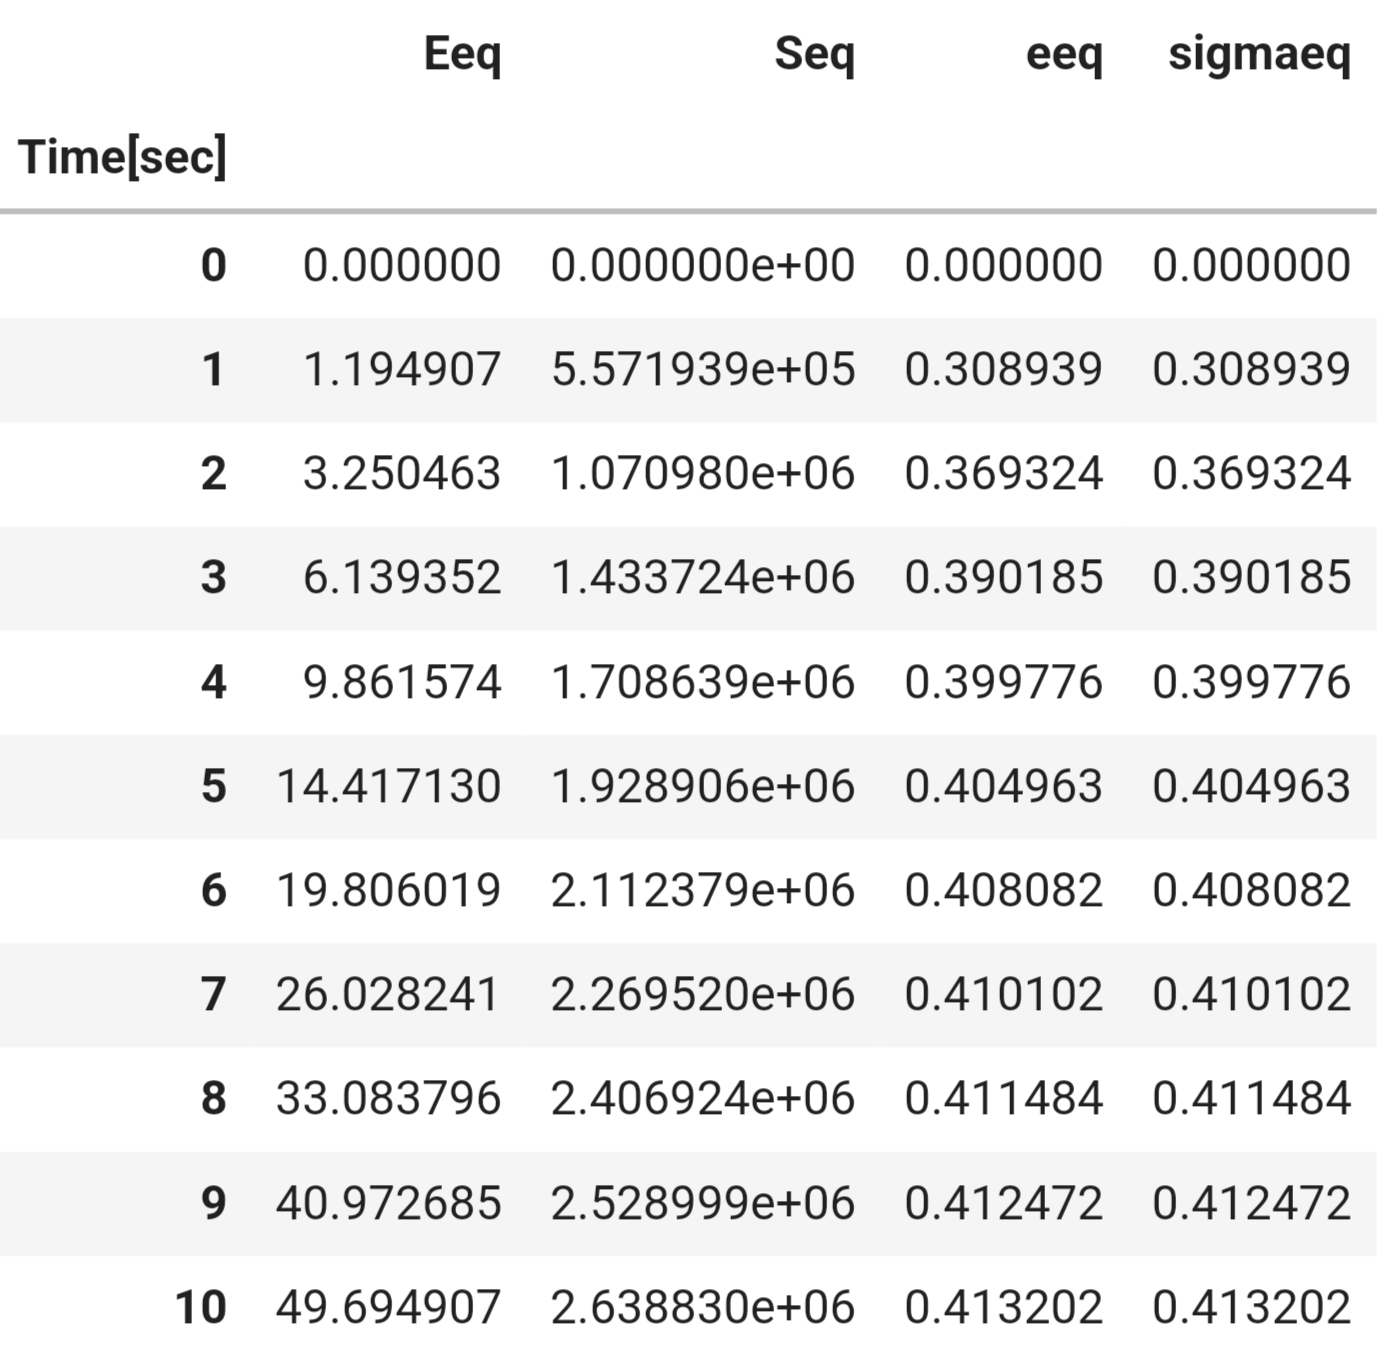
\includegraphics[width=\textwidth]{Values/m2t6.png}
        \end{block}
        \column[t]{0.48\textwidth}
        \begin{block}{\footnotesize Method-II(time integration)}
            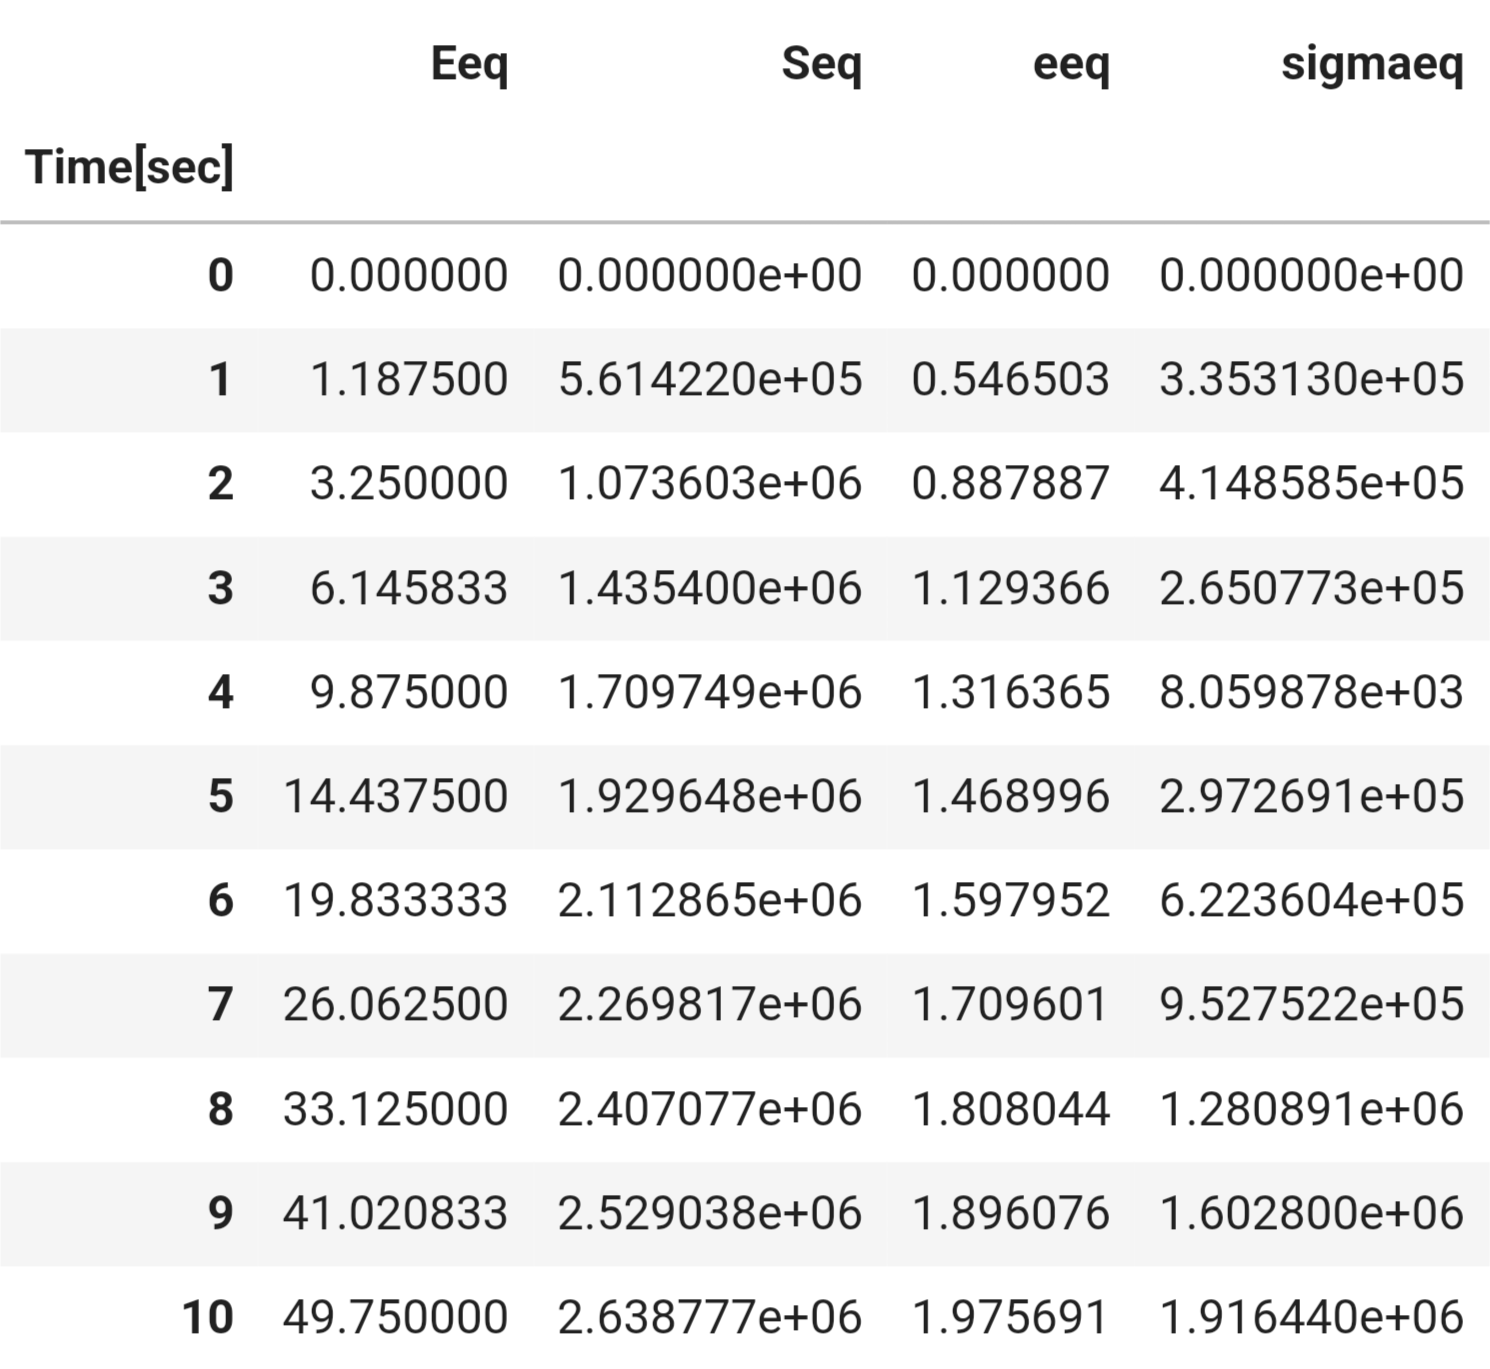
\includegraphics[width=\textwidth]{Values/m1t6.png}
        \end{block}
    \end{columns}
\end{frame}

%===================================================================
\section{Problem 7}

\begin{frame}{Problem 7 - Biaxial Compression}{Deformation and Stress vs Strain at t = 0 sec}
    \vspace{-1em}
    \scriptsize $$x_1 = X_1 - X_1t,\ x_2 = X_2 - X_2t,\ x_3 = X_3$$
    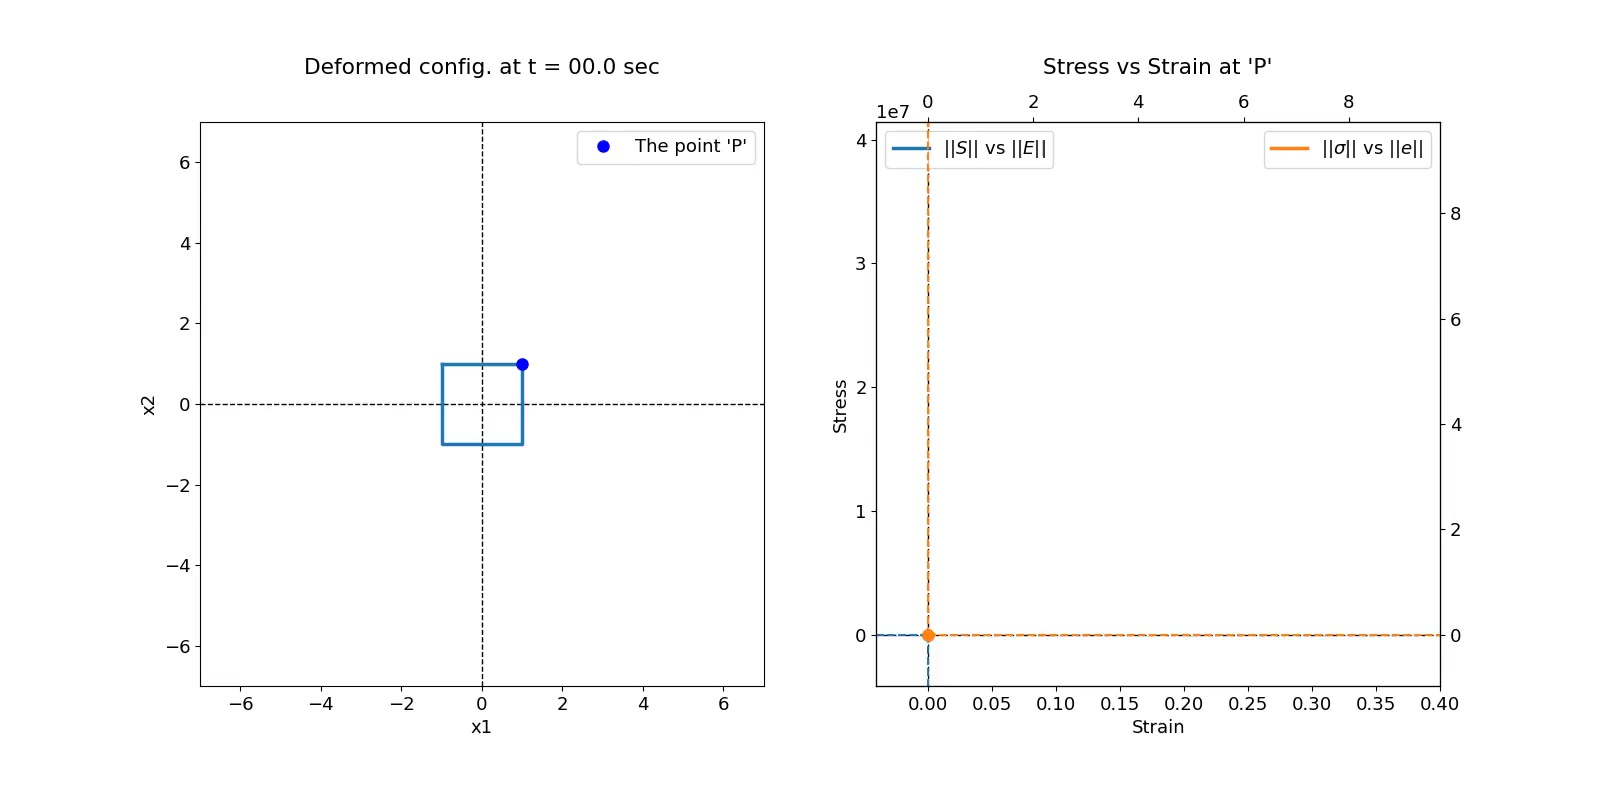
\includegraphics[width=\textwidth, trim={4.5cm 2cm 3cm 1cm}, clip]{Plots/ibicompression.jpg}
\end{frame}

\begin{frame}{Problem 7 - Biaxial Compression}{Deformation and Stress vs Strain at t = 0.8 sec}
    \vspace{-1em}
    \scriptsize $$x_1 = X_1 - X_1t,\ x_2 = X_2 - X_2t,\ x_3 = X_3$$
    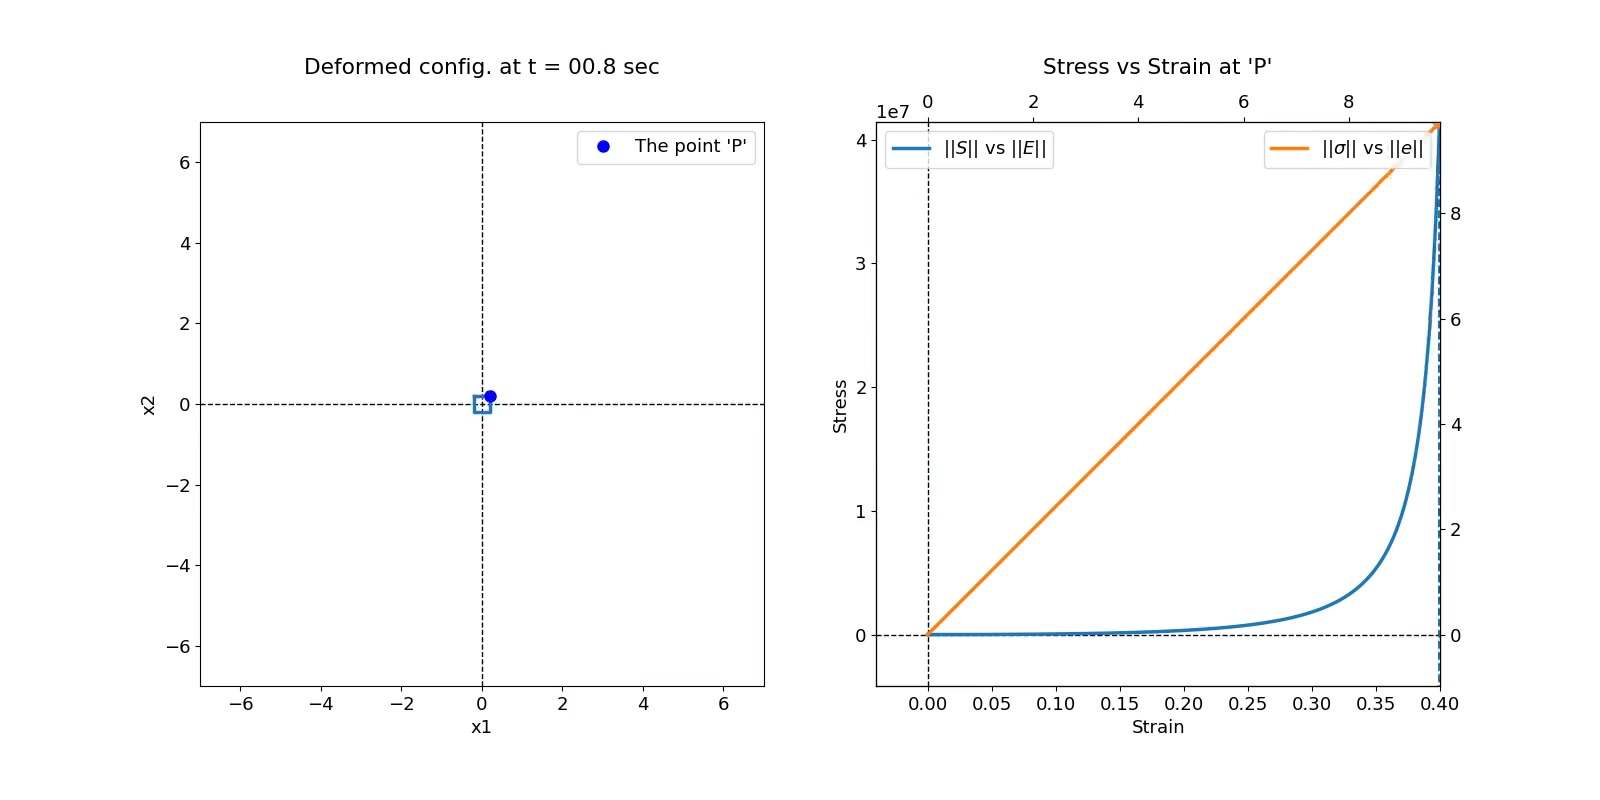
\includegraphics[width=\textwidth, trim={4.5cm 2cm 3cm 1cm}, clip]{Plots/bicompression.jpg}
\end{frame}

\begin{frame}{Problem 7 - Biaxial Compression}{Method-I vs Method-II(time integration)}
    \vspace{-2em}
    \begin{columns}
        \column[t]{0.48\textwidth}
        \begin{block}{\footnotesize Method-I}
            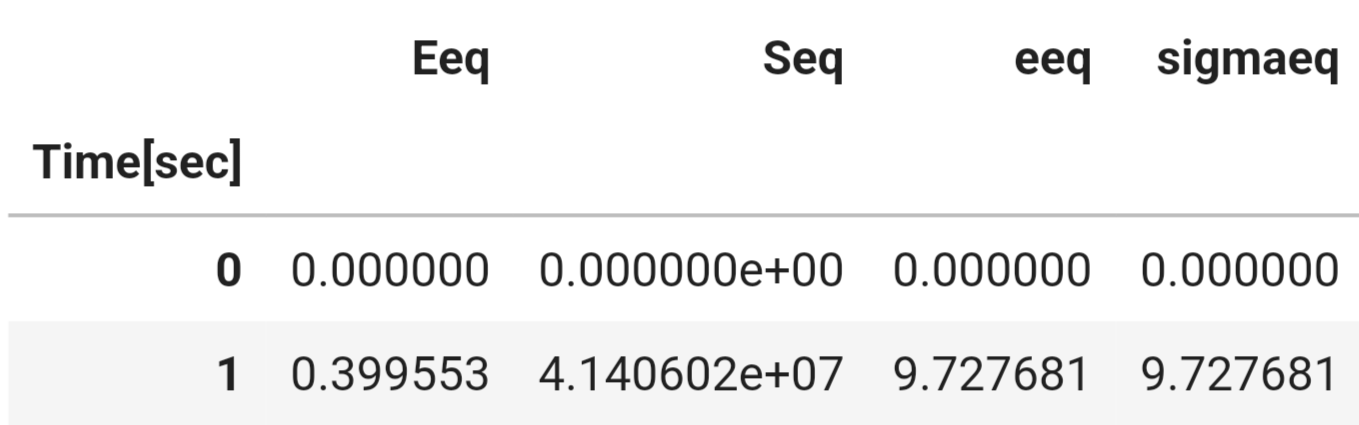
\includegraphics[width=\textwidth]{Values/m2t7.png}
        \end{block}
        \column[t]{0.48\textwidth}
        \begin{block}{\footnotesize Method-II(time integration)}
            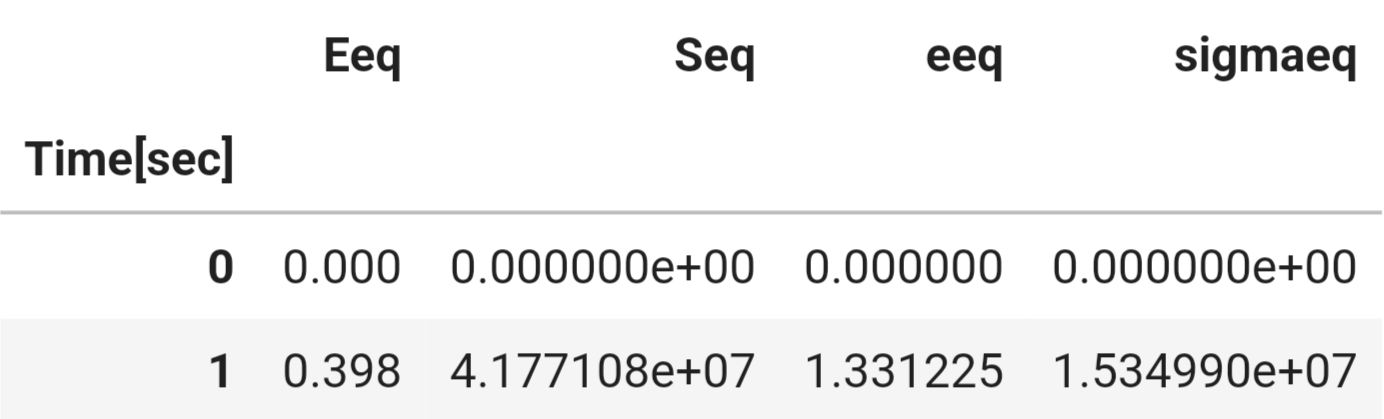
\includegraphics[width=\textwidth]{Values/m1t7.png}
        \end{block}
    \end{columns}
\end{frame}

%===================================================================
\section{Problem 8}

\begin{frame}{Problem 8 - Plane Strain Compression}{Deformation and Stress vs Strain at t = 0 sec}
    \vspace{-1em}
    \scriptsize $$x_1 = X_1 + X_1t,\ x_2 = X_2 - X_2t,\ x_3 = X_3$$
    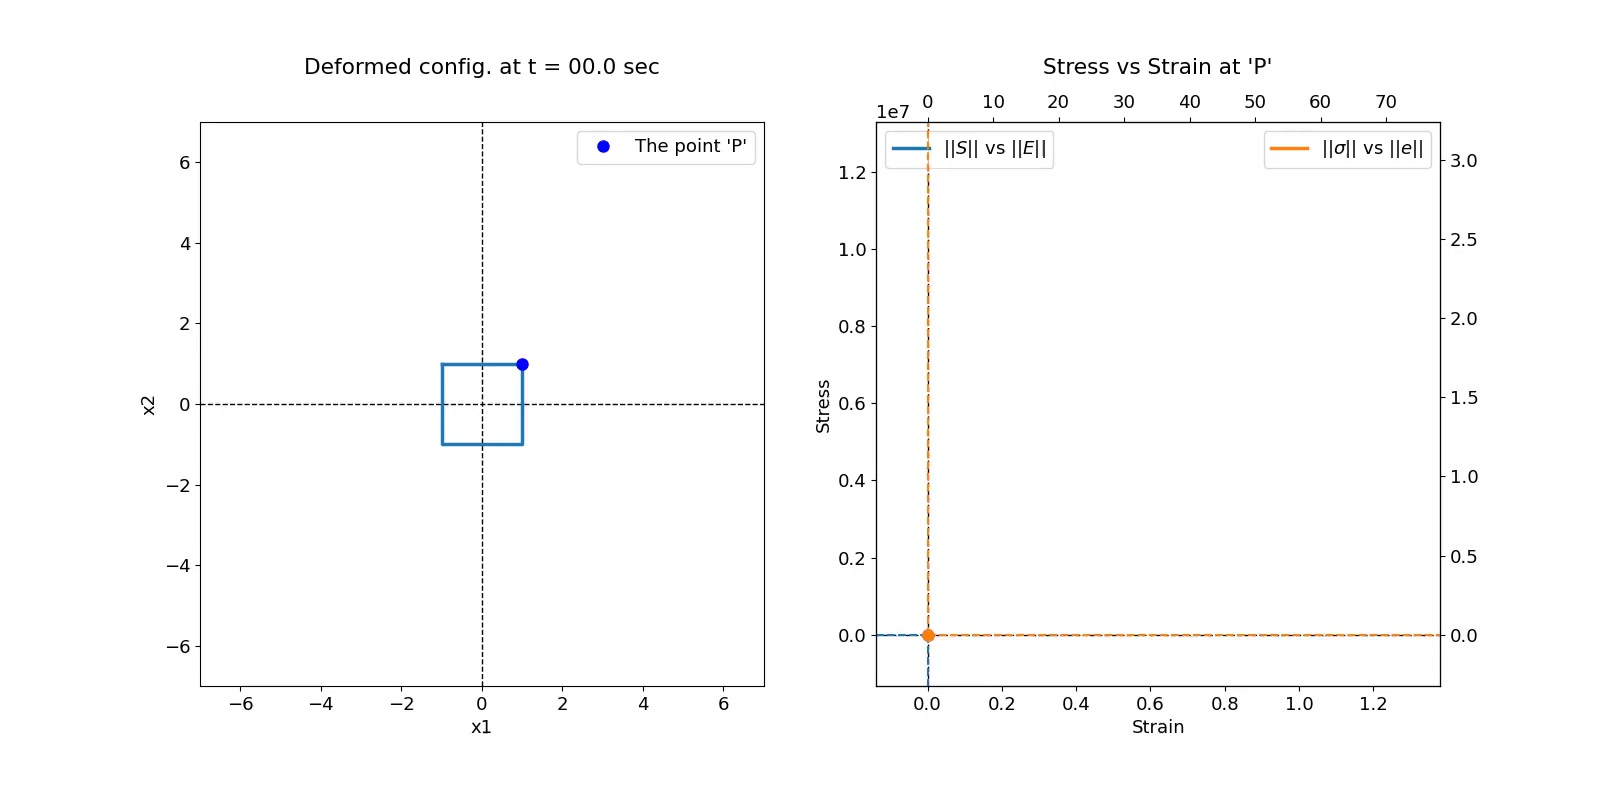
\includegraphics[width=\textwidth, trim={4.5cm 2cm 3cm 1cm}, clip]{Plots/ipscompression.jpg}
\end{frame}

\begin{frame}{Problem 8 - Plane Strain Compression}{Deformation and Stress vs Strain at t = 0.8 sec}
    \vspace{-1em}
    \scriptsize $$x_1 = X_1 + X_1t,\ x_2 = X_2 - X_2t,\ x_3 = X_3$$
    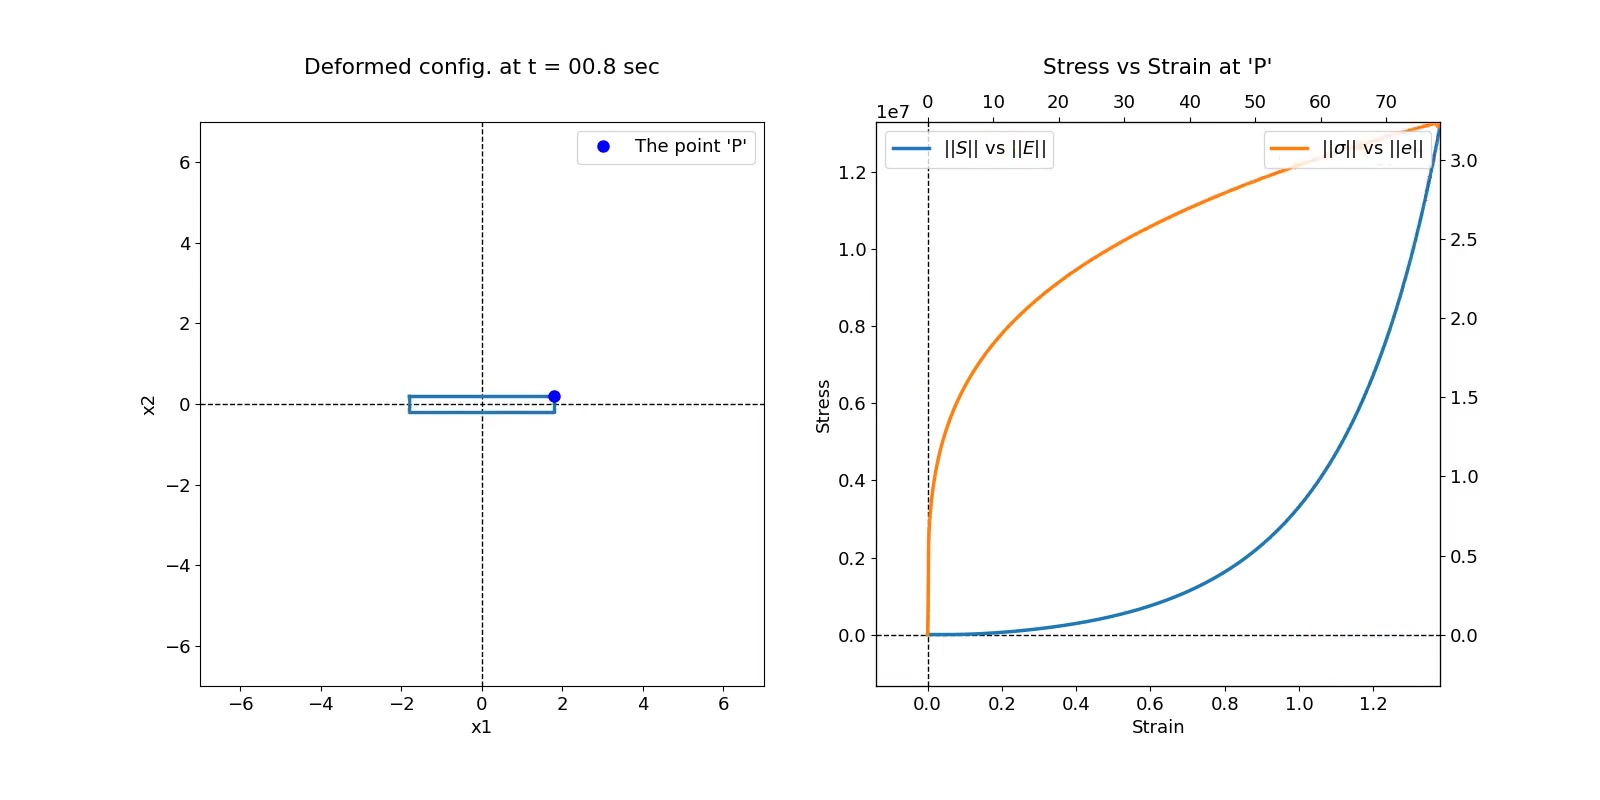
\includegraphics[width=\textwidth, trim={4.5cm 2cm 3cm 1cm}, clip]{Plots/pscompression.jpg}
\end{frame}

\begin{frame}{Problem 8 - Plane Strain Compression}{Method-I vs Method-II(time integration)}
    \vspace{-2em}
    \begin{columns}
        \column[t]{0.48\textwidth}
        \begin{block}{\footnotesize Method-I}
            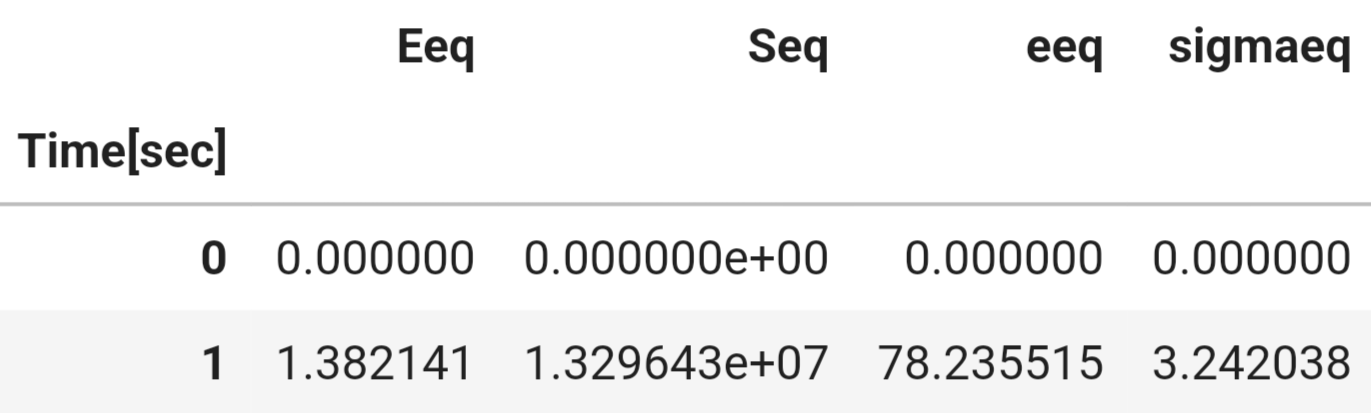
\includegraphics[width=\textwidth]{Values/m2t8.png}
        \end{block}
        \column[t]{0.48\textwidth}
        \begin{block}{\footnotesize Method-II(time integration)}
            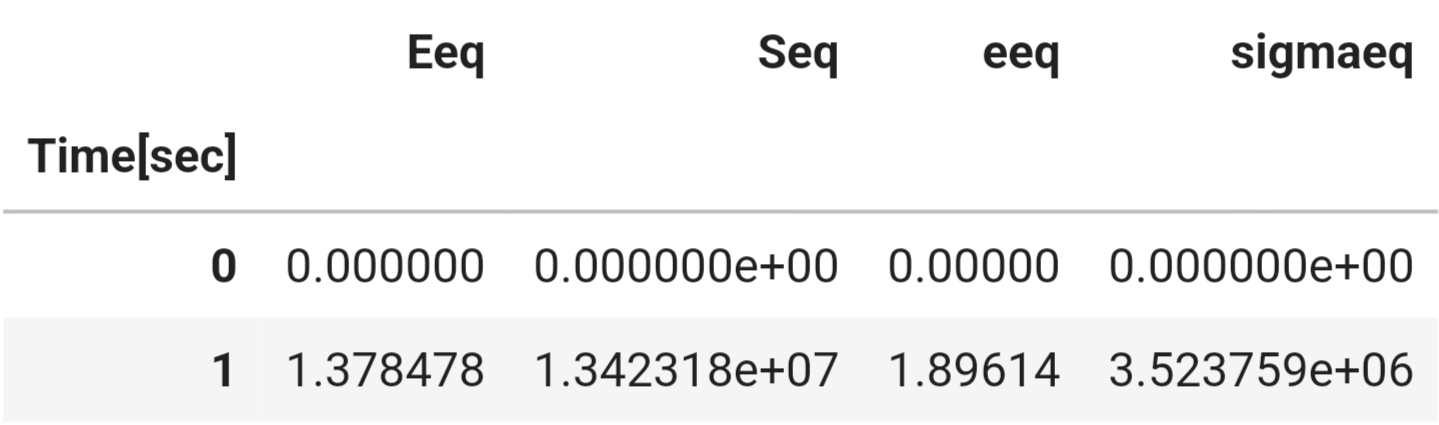
\includegraphics[width=\textwidth]{Values/m1t8.png}
        \end{block}
    \end{columns}
\end{frame}

%===================================================================
\section{Conclusions}

\begin{frame}[t]{Conclusions}{Observations made from method-I and method-II(time integration)}
        \begin{block}{\footnotesize Method-I}
            \footnotesize
            \begin{enumerate}
                \item Method-I gives the required quantities at any time step directly and does not require quantities from previous time step.
                \item The accuracy of this method does not depend up on the no of time steps chosen.
            \end{enumerate}
        \end{block}
        \begin{block}{\footnotesize System of nonlinear equations}
            \footnotesize
            \begin{enumerate}
                \item Method-II(time integration) gives the required quantities at any time step but requires quantities from previous time step.
                \item The accuracy of this method depends up on the no of time steps chosen.
            \end{enumerate}
        \end{block}
\end{frame}

% %---------------------SLIDE---------------------------------------
% \begin{frame}{Equations of motion} 
% \begin{columns}
%     \column{0.4\textwidth}
%     \begin{block}{Newton's second law}
%    $m\ddot{x} = F(\dot{x}, x, t)$
%     \end{block}
%     \begin{block}{Schrödinger's equation}
%     ${\displaystyle i\hbar {\frac {d}{dt}}\vert \Psi (t)\rangle ={\hat {H}}\vert \Psi (t)\rangle }$
%     \end{block}
%     \begin{block}{Ampère's circuital law}
%     $ \nabla \times \mathbf{B}=\frac{1}{c}\left(4 \pi \mathbf{J}+\frac{\partial \mathbf{E}}{\partial t}\right)$
%     \end{block}
% \end{columns}
% \end{frame}
% %---------------------SLIDE---------------------------------------
% \begin{frame}{Important question}
%     Important question again
% \end{frame}
% %---------------------SLIDE---------------------------------------
% \section{Important section}
% \begin{frame}{Bullet points}
% \begin{itemize}
%     \item Item A
%     \item Item B
%     \item Item C
% \end{itemize}
% \end{frame}
% %---------------------SLIDE---------------------------------------
% \begin{frame}{Using pause}
% This is a sentence. \pause 
% And this too. \pause
% \alert{Bye}. 
% \end{frame}

% %---------------------SLIDE--------------------------------------
% \begin{frame}{A Theorem}
% \begin{theorem}[Freshman's Dream] 
%  $(a+b)^p \equiv a^p + b^p \, (mod \,p)$ if p is a prime number.
% \end{theorem} \pause
% \begin{proof}
% A valid proof.
% \end{proof}
% \begin{example}
% Maybe an example?
% \end{example}
% \end{frame}

% %-----------------------------SLIDE --------------------------------------

% %Below must be compiled using LuLaTex (for emoji package):

% % \begin{frame}{Summary}

% % \begin{itemize}
% %     \item[\emoji{check-mark-button}] Concept A
% %      \item[\emoji{check-mark-button}] Concept B
% %      \item[\emoji{check-mark-button}] Concept C
% % \end{itemize}
% % \end{frame}


% %-----------------------------SLIDE --------------------------------------

% \begin{frame}{How do you write a thesis?}

% \begin{enumerate}
%     \item Eat
%     \item Sleep
%     \item Rave
%     \item Repeat
% \end{enumerate}
% \end{frame}


% %-----------------------------SLIDE --------------------------------------

% \begin{frame}{Frame title}{Frame subtitle}
% This is how you can cite \cite{Dirac}.
% \end{frame}
% %-----------------------------SLIDE --------------------------------------
% \begin{frame}{The end.}
% \begin{columns}
% \column{0.4\textwidth}
% This is a column.

% \column{0.4\textwidth}
% 
\includegraphics[width=0.9\textwidth]{Figures/meme.png}    
% \end{columns}    
    
    
% \end{frame}

% %---------------------------------------------------------
% \section{References}
% \begin{frame}[allowframebreaks]\frametitle{References}
%         \bibliographystyle{apalike}
%         \bibliography{bib}
% \end{frame}


\end{document}